\documentclass[a4paper, 11pt, oneside]{scrartcl}
\usepackage{lpp}
\usepackage{graphicx}
\usepackage{tikz}
\usetikzlibrary{shapes.geometric, arrows}

\begin{document}

\mtitle{Unstructured FEM: Final Report}

\mauthor{Mohsin Ali Chaudry, Raghavan Lakshmanan, Abhishek Y. Deshmukh}{A. Emre Ongut}

\maff{SiSc Laboratory}{a.deshmukh@grs-sim.de}{ongut@cats.rwth-aachen.de}

\mabstract{This engineering project of SiSc Lab involves the development of a parallel finite element
solver that uses unstructured grids. The developed and optimized serial code is validated using
analytical solutions and then it is parallelized and used to solve a time-dependent engineering heat
transfer problem. 
}

\section{Introduction}

\nocite{midsummer}
Finite element method(FEM) is numerical procedure that is used to obtain solutions of variety of engineering problems like stress analysis, fluid flow, heat transfer, etc. In this project, we are particularly using FEM to solve heat transfer problem for unstructured mesh for steady and unsteady 2D case.

Finite element implementation can generally be divided into following steps:

\subsection{Preprocessing}
\begin{itemize}
\item Discretization of domain into finite elements which comprises of nodes and elements
\item We then have to specify a shape function to represent physical behaviour of element
\item Construct local stiffness matrix and then ultimately global stiffness matrix
\item Then we have to apply boundary condition, initial conditions and loading (forcing function)
\end{itemize}

\subsection{Solution Phase}
\begin{itemize}
\item  Solving linear system of algebraic equations to obtain nodal results.
\end{itemize}


\subsection{PostProcessing Phase}
\begin{itemize}
\item  Postprocess the results. For instance, visualizing temeprature distribution using Paraview, generating plots by extracting relevant information.
\end{itemize}

\section{Finite Element Formulation: Unsteady State}
We are going to model transient heat diffusion equation. This model can also be used to predict the steady state if we let it run for sufficiently large time.

\subsection{1D Heat Diffusion Equation}
One dimensional unsteady heat diffusion equation with some forcing function can be written as

$$\frac{\partial T}{\partial t}-\alpha \frac{\partial^2T}{\partial x^2} =f , \text{in }  \Omega \in \Re $$ 
where $\alpha$ is diffusion coefficient.
$$ \alpha = \frac{k}{\rho c_p}$$
k is heat conductivity, $\rho$ is the density and $c_p$  is the specific heat capacity of the material.
$$ f = \frac{\dot{q}}{\rho c_p}$$
where $\dot{q}$ is heat generation per unit volume.

In order to solve this unsteady problem, we apply semi-discretization, in which forward euler method is used to discretize in time. In addition, we need two boundary conditions and one initial condition.

Here, temeprature evolves in time and space. We apply weighted residual method.

 $$\int_\Omega (w \frac{\partial T}{\partial t}  +\alpha w\frac{\partial^2 T}{\partial x^2})dx= \int_\Omega wfdx $$
 
where w is a weigthing function or test function.
Integrating by parts and rearranging the terms,
 $$\int_\Omega (w \frac{\partial T}{\partial t}  +\alpha \frac{\partial w}{\partial x}\frac{\partial T}{\partial x})dx= \int_\Omega wfdx+\int_ \Gamma (w \frac{k}{\rho c_p} \frac{\partial T}{\partial x}n_x)d \Gamma $$
\begin{figure}[ht!]
\centering
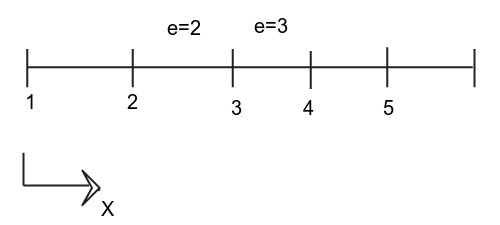
\includegraphics[width=70mm]{element.jpeg}
\caption{Stencil of element}

\end{figure}

 \textbf{Intial and Boundary Conditions:}
 
 The initial distribution of temperature over the domain $\Omega$ can be provided. 
 $$T(x,0) = T_{initial}(x)$$
 
 Boundary conditions can be of three types:

 Dirichlet: $$T(0,t) = T_L$$ $$T(L,t) = T_R$$ where temperature at boundary nodes is known.


 Neumann: $$k\frac{\partial T}{\partial x} n_x = q_0$$ where heat flux going in or out of the boundary is known.


 Robin(Mixed): $$h(T - T_{\infty}) = -k\frac{\partial T}{\partial x}$$ where the temperature of the free stream fluid ($T_{\infty}$) and correspoding heat transfer coefficient(h) is known.
 
\begin{itemize}
\item Approximate solution: We approximate the temperature as a piecewise linear combination of shape functions $S_j(x)$. These shape functions remain constant over time, so the coefficients $T_j(t)$ are time dependent.
 \end{itemize}
 $${ T }_{ app }(x,t)=\sum _{ j=1 }^{ nn }{ { T }_{ j }(t){ S }_{ j }(x) } $$
 
\begin{figure}
\centering
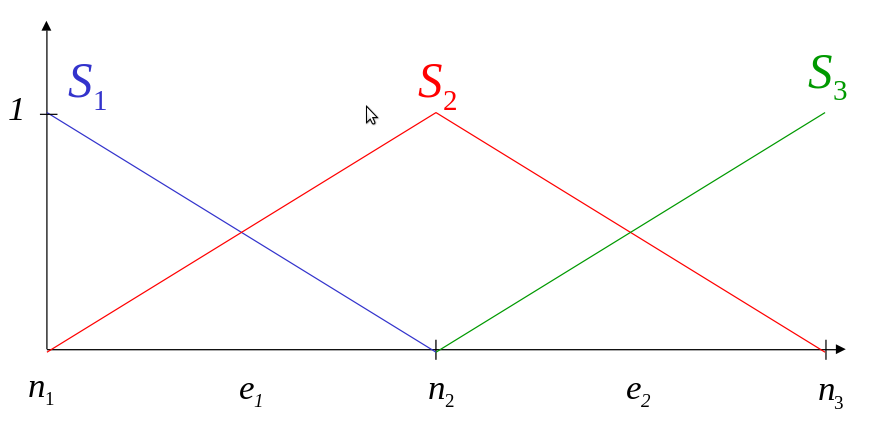
\includegraphics[scale=0.3]{./hat_fun.png}
\caption{Shape functions}
\end{figure}
$$ \int_\Omega [w\sum_{j=1}^{nn} \frac{dT_j}{dt}S_j +\alpha \frac{dw}{dx}(\sum_{j=1}^{nn}T_j\frac{dS_j}{dx})]dx=\int_\Omega wfdx+\frac{1}{\rho c_p}\int_\Gamma w(k\frac{\partial T}{\partial x})d\Gamma$$

\begin{itemize}
\item Galerkin Finite Element Method: Here weight functions are taken as $$w=S_i(x)$$
\end{itemize}
$$\int_\Omega [S_i\sum_{j=1}^{nn} \frac{dT_j}{dt}S_j +\alpha \frac{dS_i}{dx}(\sum_{j=1}^{nn}T_j\frac{dS_j}{dx})]dx=\int_\Omega S_ifdx+\frac{1}{\rho c_p}\int_\Gamma S_i(k\frac{\partial T}{\partial x})d\Gamma$$

By taking summation outside of integral for i=1,2,...,nn
$$\underbrace{\sum_{j=1}^{nn} \int_\Omega (S_i S_j)dx\frac{dT_j}{dt}}_{[M][\dot T]} +\underbrace{\sum_{j=1}^{nn}[\int_\Omega(\alpha \frac{dS_i}{dx}\frac{dS_j}{dx})dx]T_j}_{[K][T]}=\underbrace{\int_\Omega S_ifdx}_{[F]} + \underbrace{\frac{1}{\rho c_p}\int_\Gamma S_i(k\frac{\partial T}{\partial x})d\Gamma}_{[B]}$$

In matrix form we can write it as:
$$[M][\dot{T}]+[K][T]=[F]+[B]$$

Forward Euler explicit differencing in time:

$$ \frac{dT}{dt } \mid_s = \frac{T^{s+1}-T^s}{ \Delta t} +O( \Delta t)$$

$$[M]  \frac{[T]^{s+1}-[T]^s}{ \Delta t} +[K][T]^s=[F]+[B]$$

$$[M] [T]^{s+1}=[M][T]^s+{ \Delta t} ([F]+[B]-[K][T]^s)$$


Backward Euler, Implicit differencing in time:

$$ \frac{dT}{dt } \mid_{s+1} = \frac{T^{s+1}-T^s}{ \Delta t} +O( \Delta t)$$

$$ [M]\frac{T^{s+1}-T^s}{ \Delta t} +[K][T]^{s+1}=[F]+[B]$$

$$[M] [T]^{s+1}=[M][T]^s+{ \Delta t} ([F]+[B]-[K][T]^{s+1})$$

Stencil in time can be viewed as :

\begin{figure}[ht!]
\centering
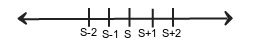
\includegraphics[width=70mm]{stencil.jpeg}
\caption{Time level stencil}

\end{figure}

We use forward euler differencing scheme here.


$$\left[ M \right] { \left[ T \right]  }^{ s+1 }=\left[ M \right] { \left[ T \right]  }^{ s }+\Delta t(\left[ F \right] +\left[ B \right] -\left[ K \right] { \left[ T \right]  }^{ s })$$

$$\begin{pmatrix} * & * & \quad  & \quad  & \quad  \\ \quad * & * & * & \quad  & \quad \quad  \\ \quad  & * & M & * & \quad  \\ \quad  & \quad  & * & * & * \\ \quad  & \quad  & \quad  & * & * \end{pmatrix}\\ \quad {\begin{bmatrix} T_{ 1 } \\ . \\ . \\ . \\  T_{ nn } \end{bmatrix} }^{ s+1 }=\begin{pmatrix} * & * & \quad  & \quad  & \quad  \\ \quad * & * & * & \quad  & \quad \quad  \\ \quad  & * & M & * & \quad  \\ \quad  & \quad  & * & * & * \\ \quad  & \quad  & \quad  & * & * \end{pmatrix}\\ \quad {\begin{bmatrix} T_{ 1 } \\ . \\ . \\ . \\  T_{ nn } \end{bmatrix} }^{ s } + .. $$


$$.. \Delta t({\begin{bmatrix} F_{ 1 } \\ . \\ . \\ . \\ . \\  F_{ nn } \end{bmatrix} } + {\begin{bmatrix} T_{ L } \\ . \\ . \\ . \\ . \\  T_{ R } \end{bmatrix} }- \begin{pmatrix} 1 & 0 & 0  & \quad  & \quad  \\ \quad * & * & * & \quad  & \quad \quad  \\ \quad  & * & K & * & \quad  \\ \quad  & \quad  & * & * & * \\ \quad  & \quad  & \quad  & 0 & 1 \end{pmatrix}\\ \quad {\begin{bmatrix} T_{ L } \\ . \\ . \\ . \\ . \\  T_{ R } \end{bmatrix} }^{ s }) $$

This generally results in a linear system with sparse mass matrix M on the left hand side and a right hand side. On solving this system, we can predict the temperature values at nodes at the time level $s+1$
$$[M][T]^{s+1} = [RHS]^{s}$$
The inversion of Mass matrix can be avoided if we do a physical approximation. This procedure is called lumping of mass matrix.

Lumped mass matrix

Consistent element  mass matrix $$[M_{cij}]$$
Lumped element mass matrix $$[M_{Lij}]$$	

We scale diagonal elements of consistent  mass matrix such that the total mass 	remains same.

$${ M }_{ Lii }={ M }_{ cii }\frac { \sum _{ i=1 }^{ n }{ \sum _{ j=1 }^{ n }{ { M }_{ cij } }  }  }{ \sum _{ j=1 }^{ n }{ { M }_{ cjj } }  }$$	  

This is correct only for linear elements.

\subsection{2D heat Diffusion Equation}
Two dimensional unsteady heat diffusion equation with some forcing function can be written as

$$\frac{\partial T}{\partial t}-\alpha \nabla^2T =f , \text{in }  \Omega \in \Re^2 $$ 
where $\alpha$ is diffusion coefficient.

Similar to 1D formulation, we apply weighted residual method.

 $$\int_\Omega (w \frac{\partial T}{\partial t}  +\alpha w\nabla^2T)d\Omega= \int_\Omega wfd\Omega $$
 
where w is a weigthing function or test function.
Integrating by parts and applying Gauss divergence theorem,
 $$\int_\Omega (w \frac{\partial T}{\partial t}  +\alpha \nabla w .\nabla T)d\Omega = \int_\Omega wfd\Omega + \frac{1}{\rho c_p}\int_ \Gamma w\underbrace{(k \hat{n}.\nabla T)}_{k(n_x\frac{\partial T}{\partial x} + n_y\frac{\partial T}{\partial y})}d\Gamma $$

Again, we approximate the temperature as a piecewise linear combination of shape functions $S_j(x,y)$. These shape functions remain constant over time, so the coefficients $T_j(t)$ are time dependent.

 $${ T }(x,y,t)=\sum _{ j=1 }^{ nn }{ { T }_{ j }(t){ S }_{ j }(x,y) } $$

Galerkin Finite Element Method: $$w=S_i(x)$$

$$\sum_{j=1}^{nn} \int_\Omega (S_i S_j)d\Omega \frac{\partial T_j}{\partial t} - \sum_{j=1}^{nn}[\int_\Omega \alpha (\frac{\partial S_i}{\partial x}\frac{\partial S_j}{\partial x} + \frac{\partial S_i}{\partial y}\frac{\partial S_j}{\partial y})d\Omega] T_j = \int_\Omega S_i	f d\Omega  +  \frac{1}{\rho c_p} \int_\Gamma S_i (k \hat{n}.\nabla T) d\Gamma$$
$$K_{ij} = \int_\Omega \alpha (\frac{\partial S_i}{\partial x}\frac{\partial S_j}{\partial x} + \frac{\partial S_i}{\partial y}\frac{\partial S_j}{\partial y})d\Omega$$
$i,j = 1,2,...,nn $

\textbf{2D Master Element:}

In 2D, two types of elements can be used, namely, triangular or quads depending on the mesh being used to solve upon. We have implemented for tri-elements.
\begin{figure}[ht!]
\centering
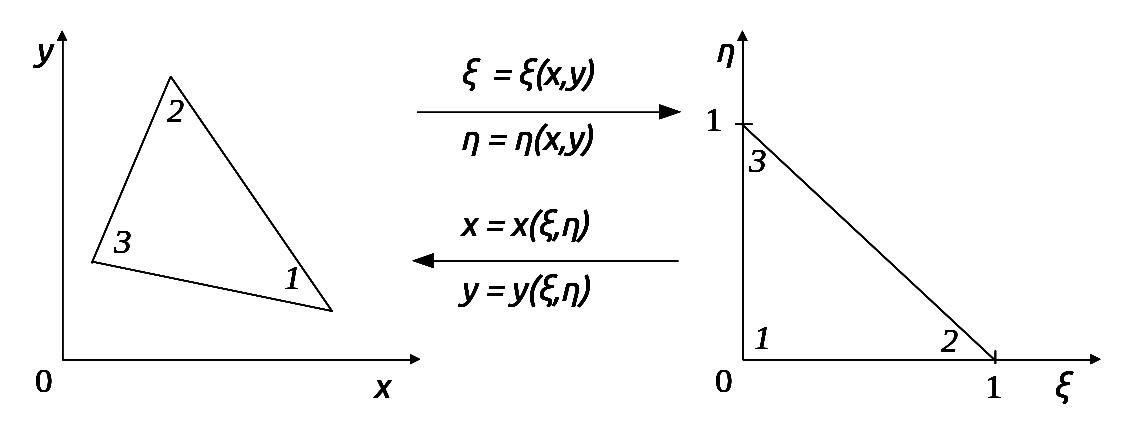
\includegraphics[width=140mm]{master_elem.png}
\caption{Co-ordinate transformation}
\end{figure}

$$S_1(\xi,\eta) = 1 - \xi - \eta$$ $$S_2(\xi,\eta) = \xi$$ $$S_3(\xi,\eta) = \eta$$

$$\frac{\partial S_1}{\partial \xi} = -1  ,    \frac{\partial S_2}{\partial \xi} = 1 ,   \frac{\partial S_3}{\partial \xi} = 0,   \frac{\partial S_1}{\partial \eta} = -1,    \frac{\partial S_2}{\partial \eta} = 0,     \frac{\partial S_3}{\partial \eta} = 1$$

$$\frac{\partial S_i}{\partial \xi} = \frac{\partial S_i}{\partial x}\frac{\partial x}{\partial \xi} + \frac{\partial S_i}{\partial y}\frac{\partial y}{\partial \xi}, \frac{\partial S_i}{\partial \eta} = \frac{\partial S_i}{\partial x}\frac{\partial x}{\partial \eta} + \frac{\partial S_i}{\partial y}\frac{\partial y}{\partial \eta}$$

$$\begin{bmatrix}
\frac{\partial S_i}{\partial \xi} \\ \\ \frac{\partial S_i}{\partial \eta}
\end{bmatrix} = \underbrace{\begin{bmatrix}
\frac{\partial x}{\partial \xi} \quad \frac{\partial y}{\partial \xi}\\ \\ \frac{\partial x}{\partial \eta} \quad \frac{\partial y}{\partial \eta} 
\end{bmatrix}}_{Jacobian} \begin{bmatrix}
\frac{\partial S_i}{\partial x} \\ \\ \frac{\partial S_i}{\partial y}
\end{bmatrix}$$

\textbf{Isoparametric formulation:}
$$x(\xi,\eta) = \sum_{j=1}^{nen} x_j^e S_j(\xi,\eta) \text{ , }
 y(\xi,\eta) = \sum_{j=1}^{nen} y_j^e S_j(\xi,\eta)$$
 Using above formulation, we can write Jacobian as:
 $$\begin{bmatrix}J\end{bmatrix} = \begin{bmatrix}
\frac{\partial S_1}{\partial \xi} \quad \frac{\partial S_2}{\partial \xi}\quad \frac{\partial S_3}{\partial \xi}\\ \\ \frac{\partial S_1}{\partial \eta} \quad \frac{\partial S_2}{\partial \eta}\quad \frac{\partial S_3}{\partial \eta} 
\end{bmatrix} \begin{bmatrix}
x_1^e \quad y_1^e\\ \\ x_2^e \quad y_2^e \\ \\ x_3^e \quad y_3^e\end{bmatrix} = \begin{bmatrix}
\frac{\partial x}{\partial \xi} \quad \frac{\partial y}{\partial \xi}\\ \\ \frac{\partial x}{\partial \eta} \quad \frac{\partial y}{\partial \eta} 
\end{bmatrix}$$
But we need $[J]^{-1}$ which is the inverse mapping. 
$$\begin{bmatrix}
\frac{\partial S_i}{\partial x} \\ \\ \frac{\partial S_i}{\partial y}
\end{bmatrix} = \underbrace{\begin{bmatrix}
\frac{\partial \xi}{\partial x} \quad \frac{\partial \eta}{\partial x}\\ \\ \frac{\partial \xi}{\partial y} \quad \frac{\partial \eta}{\partial y} 
\end{bmatrix}}_{[J]^{-1}}\underbrace{\begin{bmatrix}
\frac{\partial S_i}{\partial \xi} \\ \\ \frac{\partial S_i}{\partial \eta}
\end{bmatrix}}_{known} $$
\textbf{Calculation of element level stiffness matix:}
$$K_{ij}^e = \int_{\Omega_e} \alpha (\frac{\partial S_i}{\partial x}\frac{\partial S_j}{\partial x} + \frac{\partial S_i}{\partial y}\frac{\partial S_j}{\partial y})dx dy \text{     i,j = 1,2,...,nen}$$
Integral transformation to master element:
$$K_{ij}^e = \int_{0}^1 \int_0^{1-\xi} \underbrace{\alpha [(\frac{\partial S_i}{\partial \xi}\frac{\partial \xi}{\partial x} + \frac{\partial S_i}{\partial \eta}\frac{\partial \eta}{\partial x})(\frac{\partial S_j}{\partial \xi}\frac{\partial \xi}{\partial x} + \frac{\partial S_j}{\partial \eta}\frac{\partial \eta}{\partial x}) + (\frac{\partial S_i}{\partial \xi}\frac{\partial \xi}{\partial y} + \frac{\partial S_i}{\partial \eta}\frac{\partial \eta}{\partial y})(\frac{\partial S_j}{\partial \xi}\frac{\partial \xi}{\partial y} + \frac{\partial S_j}{\partial \eta}\frac{\partial \eta}{\partial y})]|J|}_{Integrand := f_k(\xi,\eta)}d\xi d\eta$$
$i,j = 1,2,...,nen$

The integration is done numerically using Gauss Quadrature rule. We have used 7 point Gauss Quadrature rule.
$$K_{ij}^e \simeq \sum_{l=1}^{nGQP}f_k(\xi_l,\eta_l) w_l$$

These points are shown in figure 5.
\begin{figure}[ht!]
\centering
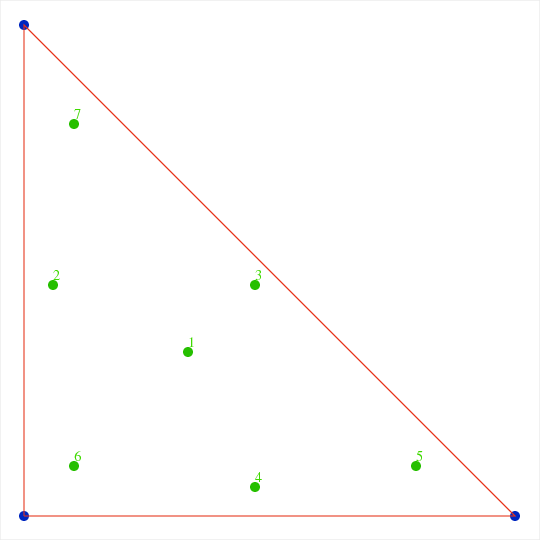
\includegraphics[width=40mm]{GQP7.png}
\caption{7 Gauss Quadrature Points}
\end{figure}
Similarly, element level mass matrix [M] and source term [S] is also calculated by numerical integration.
\\
\\
\textbf{Boundary Integral:}
\\
According to the boundary conditions, we determine the components of boundary integral. For the nodes where the essential boundary conditions($T=T_w$) are given, we don't need to evaluate the boundary integral. We can specify $T_w$ in boundary integral and make necessay changes in [K] matrix. For example, if for some element, node temperatures T1 and T3 are known then [B] and [K] for that element can be written as:
$$[B] = \begin{bmatrix}
T_w \\
B_2 \\
T_w
\end{bmatrix} \text{  and  } [K] = \begin{bmatrix}
1 \quad 0 \quad 0 \\
\ast \quad \ast \quad \ast \\
0 \quad 0 \quad 1
\end{bmatrix} $$  In addition, for the nodes on insulated wall there is no contribution to the boundary integral since the heat flux at these nodes is zero. We need to evaluate the boundary integral in case of Neumann and Robin(Mixed) boundary conditions where explicit heat flux is given. We need to evaluate this integral on the edges of the elements which lie on one of these boundaries. Over the edge the 2D shape functions reduce to 1D shape functions as it can be seen in the figure 6.\\
$S_1$ and $S_2$ can be clearly written as $S_1 = 1- \frac{r}{L}$ , $S_2 = \frac{r}{L}$
\begin{figure}[ht!]
\centering
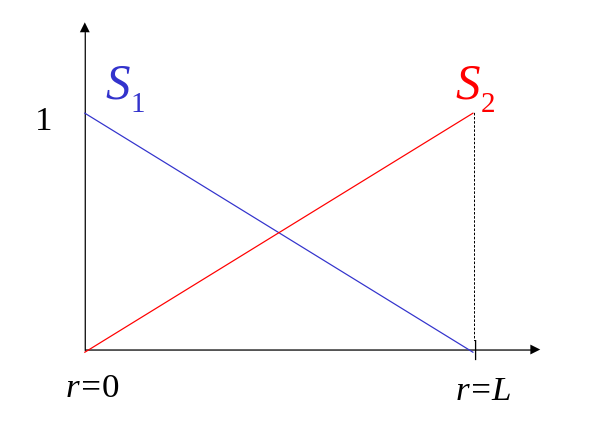
\includegraphics[width=50mm]{edge_shape_fun.png}
\caption{Shape functions over the edge of tri-element}
\end{figure}
\\
For Neumann Boundary conditions (Flux Variable(FV) = $q_{in}$):
\\
$$B_1^e = \frac{1}{\rho c_p} \int_\Gamma S_1 (FV)d\Gamma = \frac{1}{\rho c_p}\int_0^L (1-\frac{r}{L}) q_{in}dr = \frac{q_{in} L}{2 \rho c_p} $$
$$B_2^e = \frac{1}{\rho c_p} \int_\Gamma S_2 (FV)d\Gamma = \frac{1}{\rho c_p} \int_0^L \frac{r}{L} q_{in}dr = \frac{q_{in} L}{2 \rho c_p} $$

$$[B] = \begin{bmatrix}
\frac{q_{in}L}{2 \rho c_p} \\
\frac{q_{in}L}{2 \rho c_p} \\
0
\end{bmatrix}$$ 
For Robin(Mixed type) Boundary conditions:
Flux variable can be expressed as $$-k \hat{n}.\nabla T = h(T - T_{\infty})$$
$FV = a PV + b$ where a = -h and b = $hT_{\infty}$

$$B_1^e = \frac{1}{\rho c_p} \int_\Gamma S_1 (FV)d\Gamma = \frac{1}{\rho c_p} \int_0^L (1-\frac{r}{L}) (a PV + b)dr$$
$$B_2^e = \frac{1}{\rho c_p} \int_\Gamma S_2 (FV)d\Gamma = \frac{1}{\rho c_p} \int_0^L \frac{r}{L} (a PV + b)dr$$
Primary variable temperature appears inside the integrals. We can express temperature in terms of shape functions $S_1$ and $S_2$ and evaluate the boundary integrals.
$$PV = S_1 T_1 + S_2 T_2$$
$$B_1^e = \frac{1}{\rho c_p} \int_0^L (1-\frac{r}{L})[a ((1-\frac{r}{L})T_1 + \frac{r}{L}T_2 ) + b]dr = \frac{L}{6 \rho c_p}(3b + 2aT_1 + aT_2)$$
$$B_2^e = \frac{1}{\rho c_p} \int_0^L \frac{r}{L}[a ((1-\frac{r}{L})T_1 + \frac{r}{L}T_2 ) + b]dr = \frac{L}{6 \rho c_p}(3b + aT_1 + 2aT_2)$$
and element boundary vector can be written as:
$$[B] = \begin{bmatrix}
\frac{L}{6 \rho c_p}(3b + 2aT_1 + aT_2) \\
\frac{L}{6 \rho c_p}(3b + aT_1 + 2aT_2) \\
0
\end{bmatrix}$$
As the temperature which is unknown here, appears in the boundary integral, we have to rearrange [B] and [K] and transfer coefficients unknown primary variables to [K]. Modified [B] and corresponding [K] can be written as:
$$[B] = \begin{bmatrix}
\frac{Lb}{2 \rho c_p} \\
\frac{Lb}{2 \rho c_p} \\
0
\end{bmatrix} \text{  and  } [K] = \begin{bmatrix}
(\ast - \frac{aL}{3 \rho c_p}) \quad (\ast - \frac{aL}{6 \rho c_p}) \quad \quad \ast \\
(\ast - \frac{aL}{6 \rho c_p}) \quad (\ast - \frac{aL}{3 \rho c_p}) \quad \quad \ast \\
\ast \quad \quad \quad \quad \ast \quad \quad \quad \quad \ast
\end{bmatrix} $$
Rest of the procedure to evaluated the temperature at new time level from previous time level is similar to one dimenional formulation.

\section{Implementation}
 The solver has been implemented in Object Oriented C++ Code. The detailed documentation has been generated using Doxygen. Overall program flow is shown in figure 7.
% Define the styles for each block
\tikzstyle{startstop} = [rectangle, rounded corners, minimum width=3cm, minimum height=1cm,text centered, draw=black, fill=red!30]
\tikzstyle{io} = [trapezium, trapezium left angle=70, trapezium right angle=110, minimum width=3cm, minimum height=1cm, text centered, draw=black, fill=blue!30]
\tikzstyle{process} = [rectangle, minimum width=3cm, minimum height=1cm, text centered, draw=black, fill=orange!30]
\tikzstyle{decision} = [diamond, minimum width=3cm, minimum height=1cm, text centered, draw=black, fill=green!30]
\tikzstyle{arrow} = [thick,->,>=stealth]

%<TikZ code>
\begin{figure}

\begin{center}
\begin{tikzpicture}[node distance=2cm]

% Nodes
\node (start) [startstop] {Start};
\node (in1) [io, below of=start, minimum width=2cm, minimum height=1cm, text centered, text width=6cm, draw=black, yshift=-0.5cm] {Input: Mesh files, Initial and Boundary conditions, Diffusion Coefficient, Source term, No. of iterations, Time step, Data Writing Frequency};
\node (pro1) [process, below of=in1, yshift=-0.5cm] {Define Mesh Structures};
\node (pro2) [process, below of=pro1, minimum width=5cm, minimum height=1cm, text centered, text width=5cm, draw=black] {Calculate Metrics: Jacobian, Element level Matrices};
\node (pro2z) [process, below of=pro2, minimum width=4cm, minimum height=1cm, text centered, text width=3cm, draw=black] {Apply Boundary Conditions};
%\node (dec1) [decision, below of=pro1, yshift=-0.5cm] {Decision 1};
\node (pro2a) [process, below of=pro2z,  minimum width=3cm, minimum height=1cm, text centered, text width=5cm, draw=black] {Solver: Solve 2D Heat diffusion equation};
%\node (pro2b) [process, right of=pro1, xshift=2cm] {Process 2b};
\node (pro2b) [io, below of=pro2a, minimum width=3cm, minimum height=1cm, text centered, text width=2cm, draw=black] {Write VTK Data};
\node (pro2c) [process, right of=pro2b, xshift=2cm] {time+=dt};
\node (dec1) [decision, below of=pro2b, yshift=-0.5cm] {iter<NIter};
%\node (out1) [io, below of=dec1, yshift=-0.5cm, minimum width=3cm, minimum height=1cm, text centered, text width=3cm, draw=black] {Output in Paraview};
\node (stop) [startstop, below of=dec1, yshift=-0.5cm] {Stop};

% Arrows
\draw [arrow] (start) -- (in1);
\draw [arrow] (in1) -- (pro1);
%\draw [arrow] (pro1) -- (dec1);
%\draw [arrow] (dec1) -- (pro2a);
%\draw [arrow] (dec1) -- (pro2b);
\draw [arrow] (pro1) -- (pro2);
\draw [arrow] (pro2) -- (pro2z);
\draw [arrow] (pro2z) -- (pro2a);
\draw [arrow] (pro2a) -- (pro2b);
\draw [arrow] (pro2b) -- (dec1);
\draw [arrow] (dec1) -- node[anchor=east] {no} (stop);
\draw [arrow] (dec1) -| node[anchor=south] {yes} (pro2c);
\draw [arrow] (pro2c) |- (pro2a);
%\draw [arrow] (out1) -- (stop);

\end{tikzpicture}\\
\end{center}
\caption{Overall Program Flow Chart}
\end{figure}
\section{Verification}
Verification of the code is done against analytical solution found in \cite{jw}. 

\subsection{Case: 1D}
A simple 1D case is taken as an example.
Initial condition: $T_i = T(x,0) = 1000 K$
\\
Boundary Conditions: $T_L = T(0,t)) = 0$, 
$T_R = T(L,t)) = 0$, $T_{top}$ and $T_{bottom}$ are insulated
\\
Analytical Solution: $$T(x,t) = \sum_{n=1}^{\infty} B_n sin(\frac{n \pi x}{L}) e^{-\frac{n^2 \pi^2 \alpha t}{L^2}} $$ where $\alpha$ is diffusion coefficient and  $$B_n = -T_i \frac{2(-1 + (-1)^n)}{n\pi}$$

\begin{figure}[ht!]
\centering
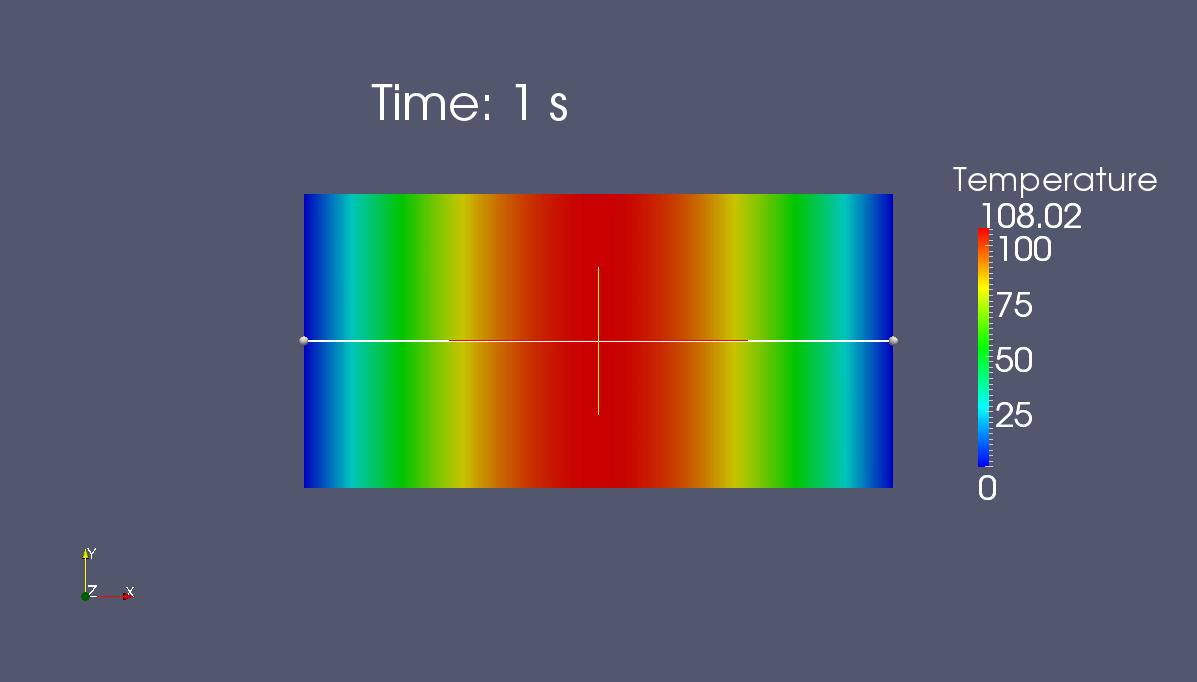
\includegraphics[width=120mm]{./Output/1D_paraview.png}
\caption{1D: Paraview Output}
\end{figure}

\begin{figure}[ht!]
\centering
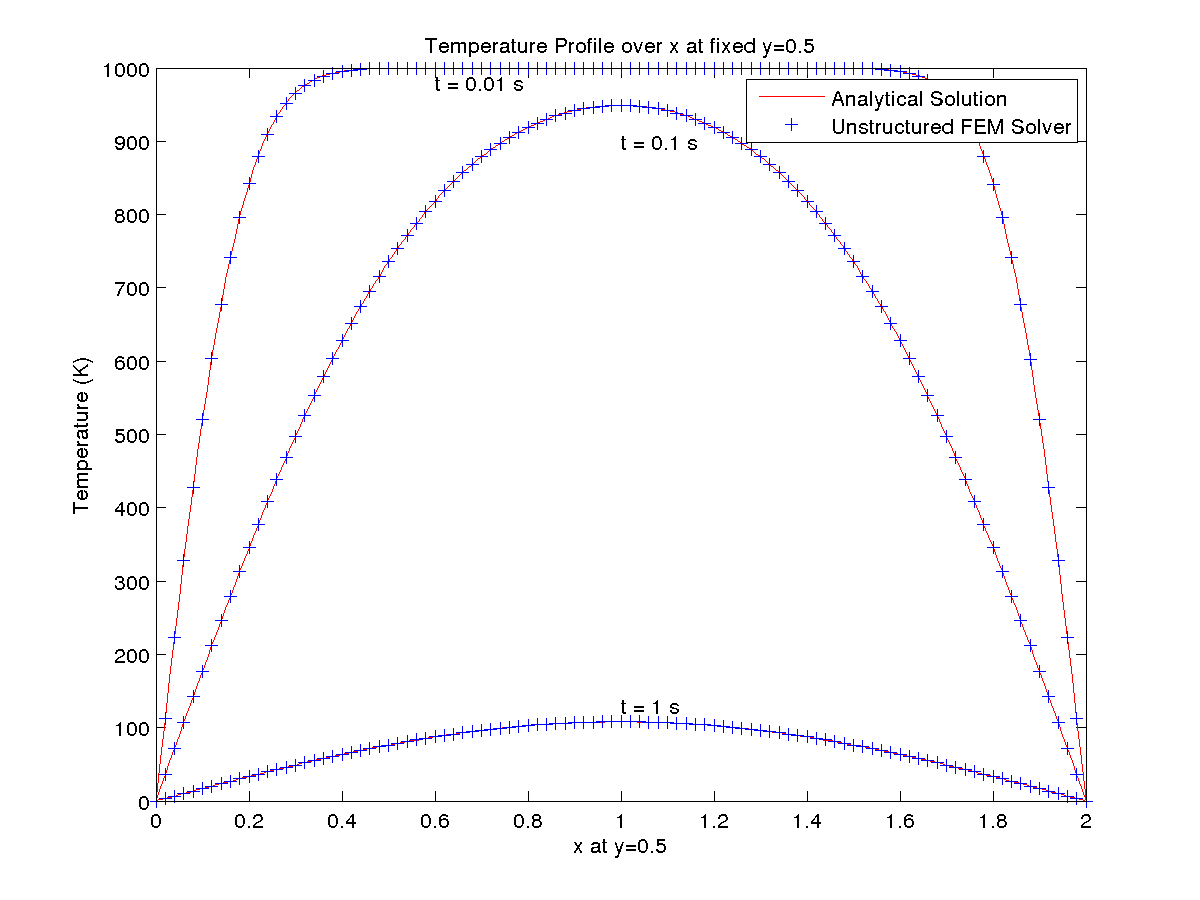
\includegraphics[width=150mm]{./Output/1D.png}
\caption{1D: Comparison with Analytical solution}
\end{figure}
As we can see from figure 9, there is excellent match of the numerical solution with analytical solution at each time level.
\subsection{Case: 2D Quenching of a Billet {\cite{jw}}}
Consider a long billet of rectangular cross section $2a \times 2b$ (a=2, b=1) initially at a uniform temperature $T_i$ which is quenched by exposing it to convective exchange with an environment at $T_{\infty}$ by means of a heat transfer coefficient h. Since the billet is long it is appropriate to neglect conduction along its axis. Because of symmetry it is enough to analyze one quarter of the cross section using a rectangular Cartesian system of coordinates with the origin at the center of the billet. 
\\
Define a shifted temperature, $\theta(x,y,t) = T(x,y,t) - T_{\infty}$
\\
Material properties: $\alpha = 1$, $\rho = 1$, $c_p = 1$, $h = 1$
\\
Initial condition: $\theta (x,y,0) = T_i - T_{\infty} = \theta_i$, $T_i = 1000$, $T_{\infty} = 300$
\\
Boundary Conditions: At $x = 0$, $$\frac{\partial \theta}{\partial x} = 0$$
At $x = a$, $$\frac{\partial \theta}{\partial x} = -\frac{h}{k} \theta (a,y,t)$$
At $y = 0$, $$\frac{\partial \theta}{\partial y} = 0$$
At $y = b$, $$\frac{\partial \theta}{\partial y} = -\frac{h}{k} \theta (x,b,t)$$
\\
In terms of the shifted temperature the analytical solution of the problem is as follows: $$\frac{\theta}{\theta_i} = 4 \sum_{n=1}^{\infty} \sum_{m=1}^{\infty} e^{(-\alpha(\lambda_n^2 + \beta_m^2) t)}\times \frac{sin(\lambda_n a) cos(\lambda_n x) sin(\beta_m b) cos(\beta_m y)}{[\lambda_n a + sin(\lambda_n a)cos(\lambda_n a)][\beta_m b + sin(\beta_m b)cos(\beta_m b)]} $$ where $\alpha$ is diffusion coefficient and  the eigenvalues $\lambda_n$ and $\beta_m$ are the roots of trancendental equations $$\lambda_n tan(\lambda_n a) = \frac{h}{k}$$ and 
$$\beta_m tan(\beta_m b) = \frac{h}{k}$$ where k is conductivity of the billet matrial.

\begin{figure}[ht!]
\centering
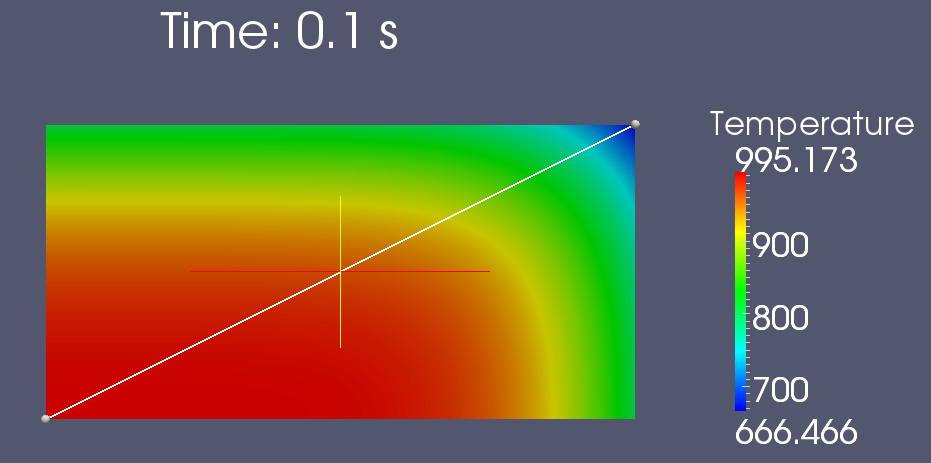
\includegraphics[width=135mm]{./Output/rsz_billet_paraview.png}
\caption{2D: Paraview Output}
\end{figure}

\begin{figure}[ht!]
\centering
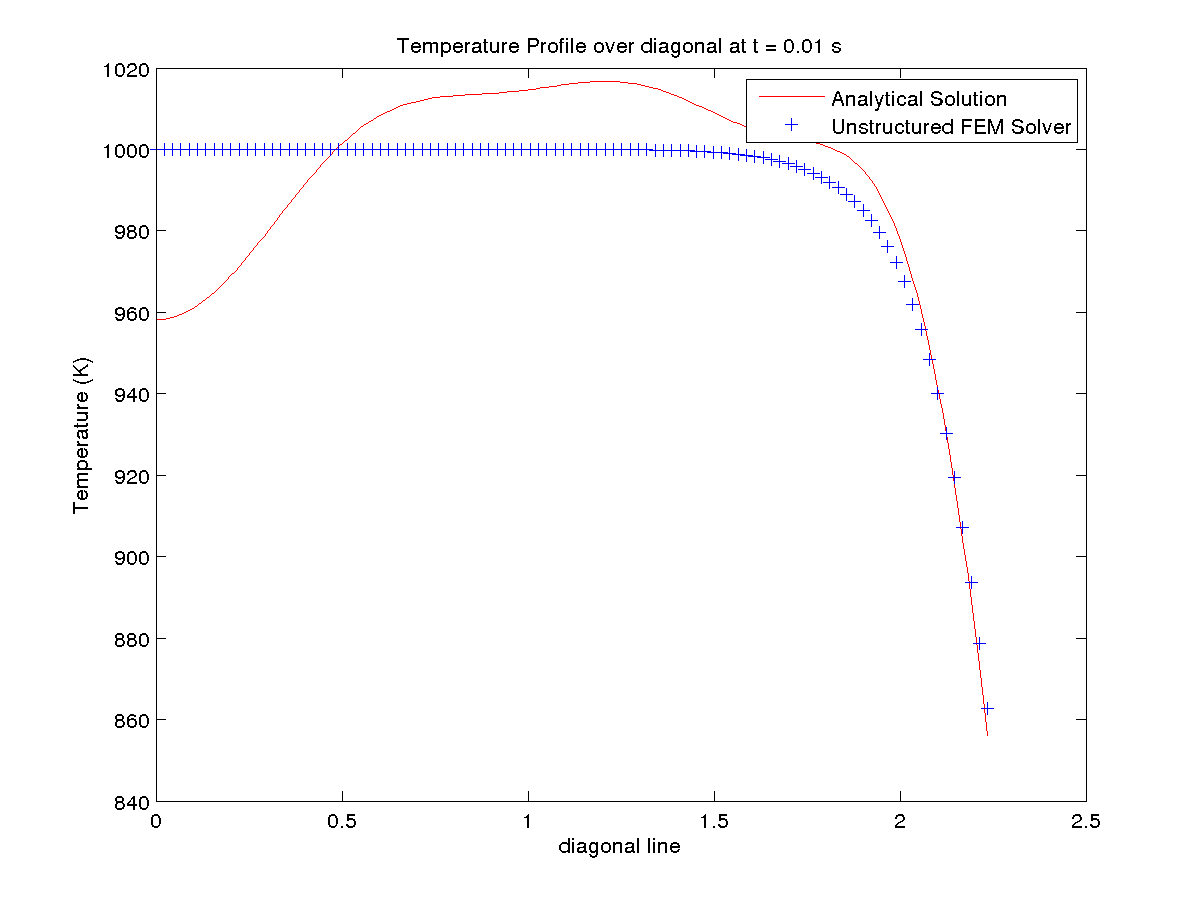
\includegraphics[width=140mm]{./Output/billet001.png}
\caption{2D: Comparison with Analytical solution at time = 0.01 s}
\end{figure}
\begin{figure}[ht!]
\centering
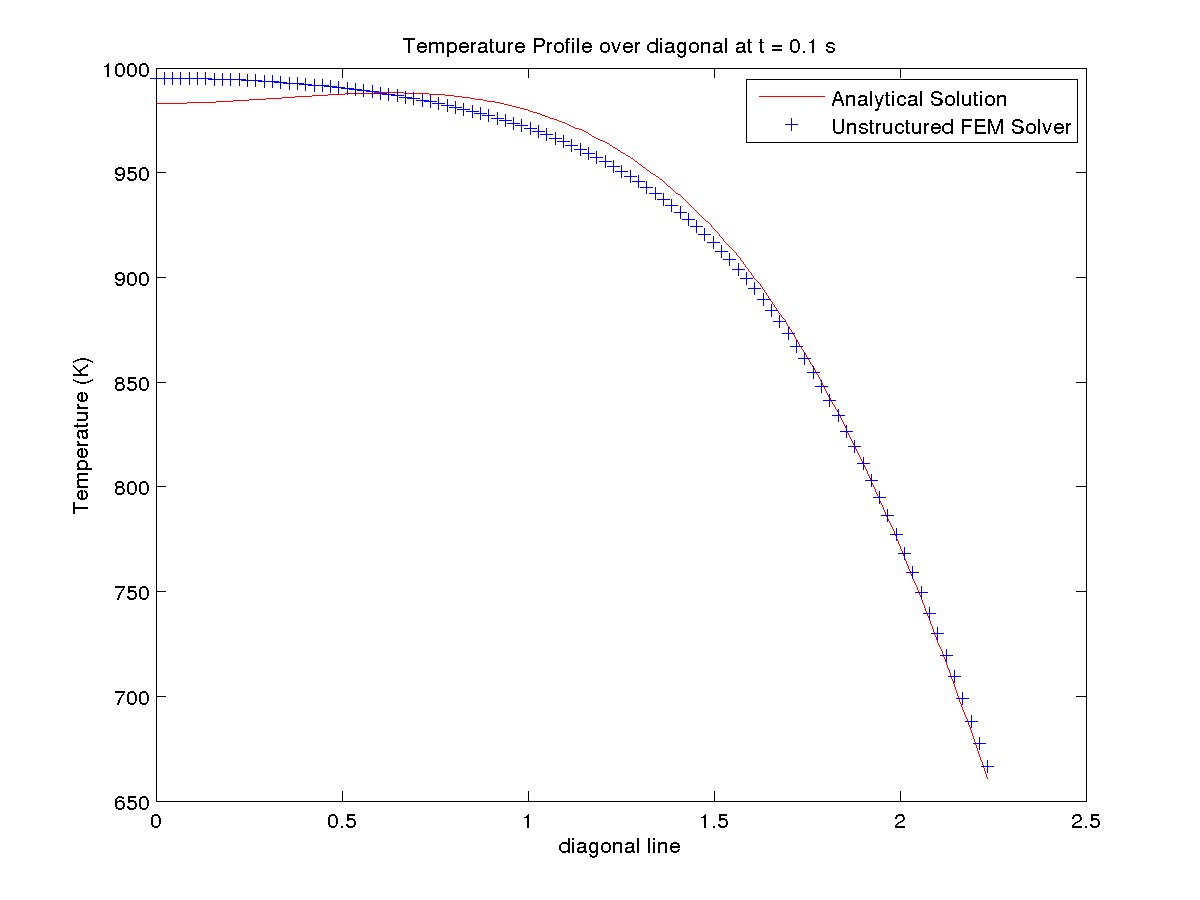
\includegraphics[width=140mm]{./Output/billet01.png}
\caption{2D: Comparison with Analytical solution at time = 0.1 s}
\end{figure}
\begin{figure}[ht!]
\centering
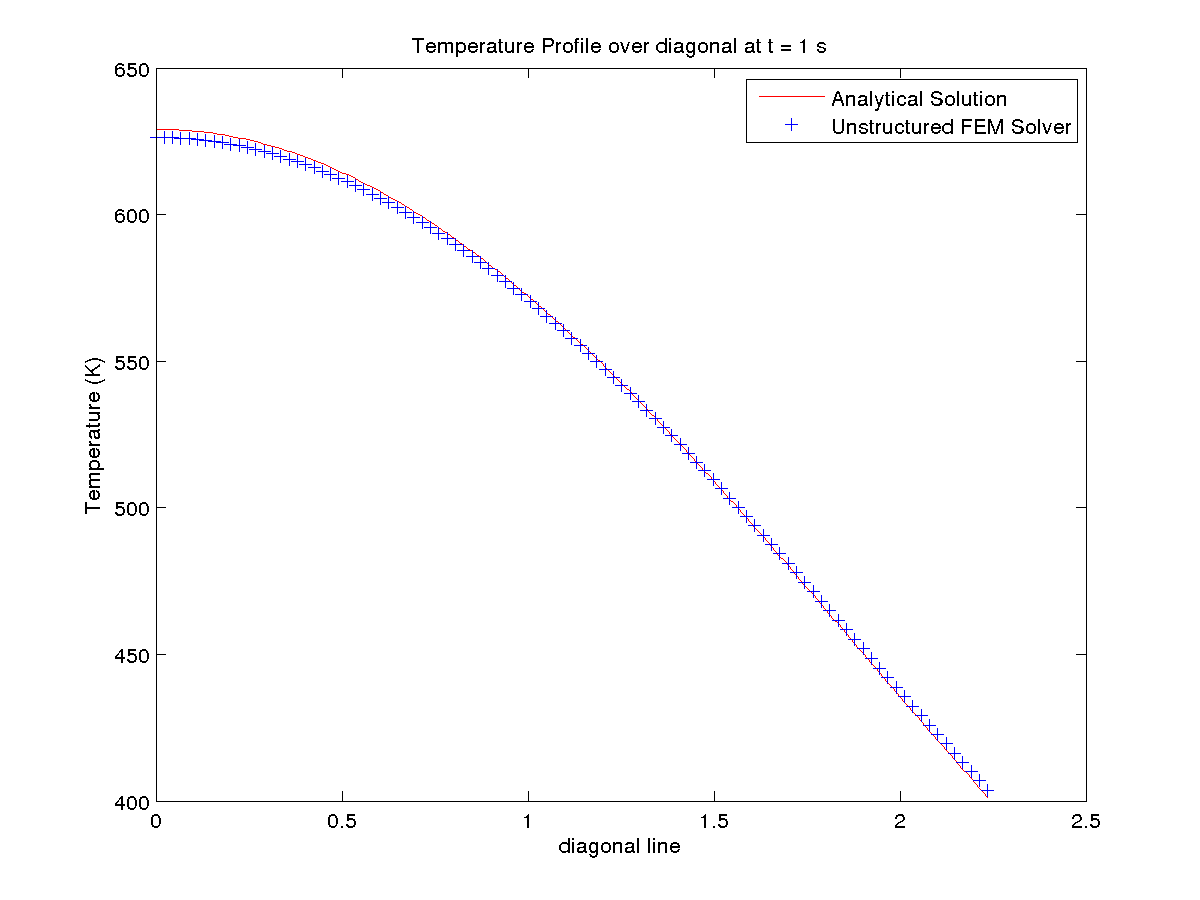
\includegraphics[width=140mm]{./Output/billet1.png}
\caption{2D: Comparison with Analytical solution at time = 1s}
\end{figure}
The plots in figures 11, 12, 13 are plotted along the white line shown in figure 10. In figure 11, the analytical solution exhibits a wavy nature. This is because the solution is in the form of Fourier series with infinite terms, but we have included finite terms for the calculation. This wavy nature is damped at higher times by the exponential factor so we can see more or less smooth behaviour in figures 12 and 13. There is good agreement between the analytical solution and numerical solution in this case too.

\section{Optimization}
Now that serial code is validated against analytical solution, the next logical step is to make it faster. One way is to optimize the code to ensure maximum cache utilization and reduce cache misses. The scalar optimization includes manually changing the code to exploit spatial and temporal locality by measures such as loop unrolling, storing reused variables as local so as to avoid cache misses, etc. There are automatic compiler optimization options such as O1, O2 and O3. We have done manual optimization wherever possible as described above and on the top of that, the highest level of automatic optimization, O3, is employed to ensure maximum performance while keeping good machine accuracy. The performance improvement can be seen in figure 14.
\begin{figure}[!htb]
\centering
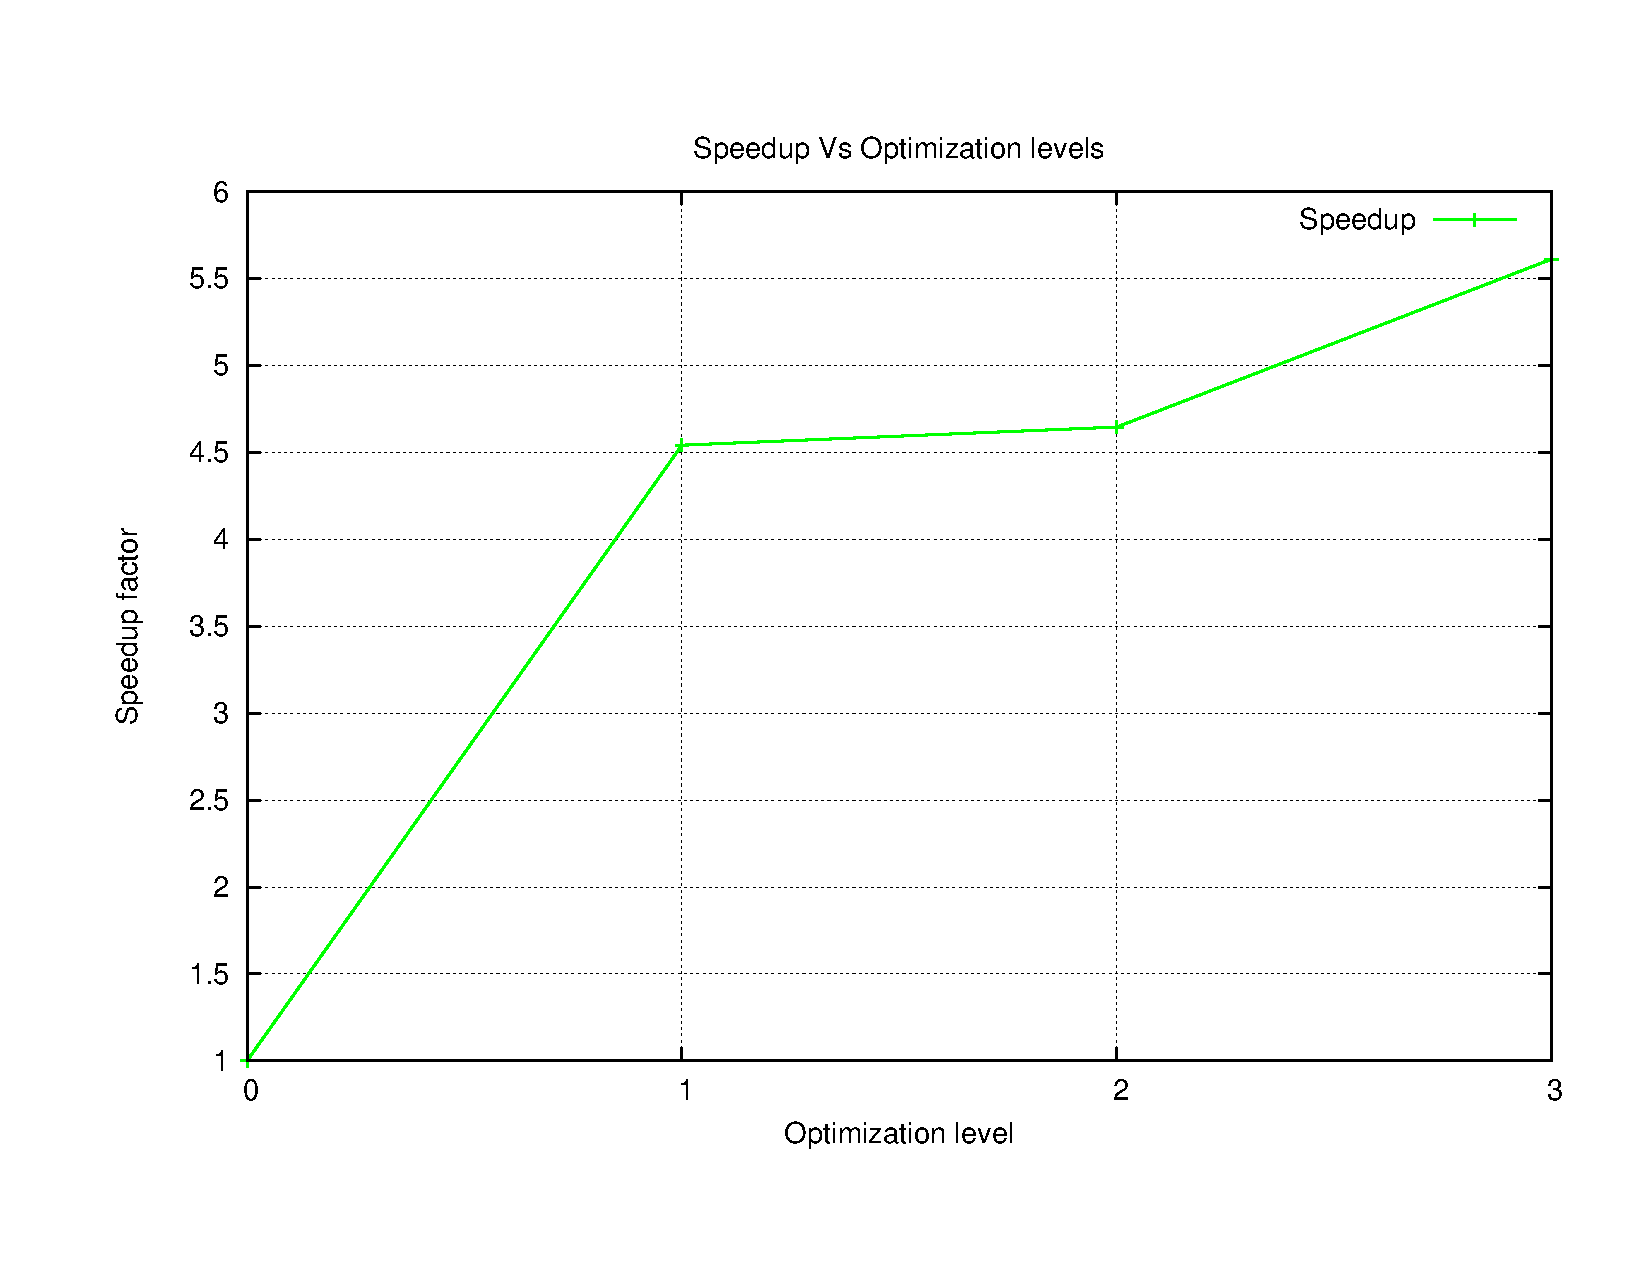
\includegraphics[scale=0.5]{./Performance.pdf}
\caption{Performance Optimization on Finemesh}
\end{figure}

\section{Parallel Computing}

Day by day the requirement for faster computing is increasing owing to increasing complexity and the size of the problems that need to be solved within stipulated amount of time. With advances in hardware hitting the atomic wall, there needs to be a way to use whatever resources are available to the maximum capacity. The large problems need to be solved fast. This motivates the use of the parallel computing that employs multiple cores to solve the problem at hand. However, the serial program needs to be significantly modified if it is to run on multiple cores. In the following sections, the approach followed by us to parallelize the serial code is described.

There are two main computing paradigms \cite{pp1}:
\begin{itemize}
\item Distributed computing
\item Multithreading
\end{itemize}

Distributed computing involves non-uniform memory access. In general, cores and memory are distributed on several machines and are connected through an interconnect. The interconnect may have different topologies like bus, radial, star, torus, omega, etc. depending on the usage. This may or may not require the processors on different machines to communicate the data required to solve the problem being considered. A standard for this communication has been developed and is called MPI (Message Passing Interface) standard.

Multithreading usually involves uniform memory access. All the cores have a shared memory from where they have access to all the data related to the problem being solved. Here, processors don't need to communicate the data. In addition multiple threads can be spawned on each core that can work on different independent piece of data and/or program. A standard for this paradigm is called OpenMP. 

There is also a hybrid paradigm that combines the distributed computing and multithreading. 

The choice of computing model depends upon the hardware available at hand. The RWTH compute cluster supports all of the above computing models. For this project, we have considered distributed computing paradigm because generally clusters with distributed resources are(or may be) readily available to the users. We want our code to be readily usable to maximum possible users who may want to use it for their problem.
\section{Approaches to Parallelizing}
The heat transfer problem to be solved involves a physical domain of interest where the temperature and heat fluxes are to be investigated. The physical domain is discretized into a mesh with triangular elements. Higher the resolution required higher will be the number of mesh elements. In parallel solution, the meshed domain can be divided into parts and each of this part can be distributed to each of the processor for solving. This is known as data parallelism. There are two ways to achieve this. Either read the mesh files namely mxyz and mien parallely or first decompose these files into required number of processors and then each processor can read parallely from its part.

Each of the approaches has its own advantages and drawbacks.

\begin{figure}[!htb]
\centering
\minipage{0.5\textwidth}
\centering
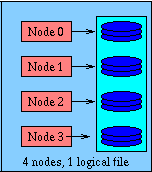
\includegraphics[]{./parallelio_0.png}
\caption{Parallel I/O 1 \cite{llnl}}
\endminipage\hfill
\centering
\minipage{0.5\textwidth}
\centering
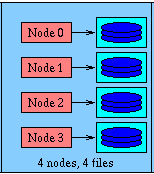
\includegraphics[]{./parallelio_1.png}
\caption{Parallel I/O 2 \cite{llnl}}
\endminipage\hfill

\end{figure}
In the first approach (Fig. 15) where processors read parallely from single mxyz and single mien file, each processor may not contain all the data related to node co-ordinates on the same processors. It requires to get missing node information from other processors (Fig. 17). This adds the communication overhead. However, there is no need to preprocess the mesh data before running the parallel code. 


\begin{figure}[!htb]
\centering
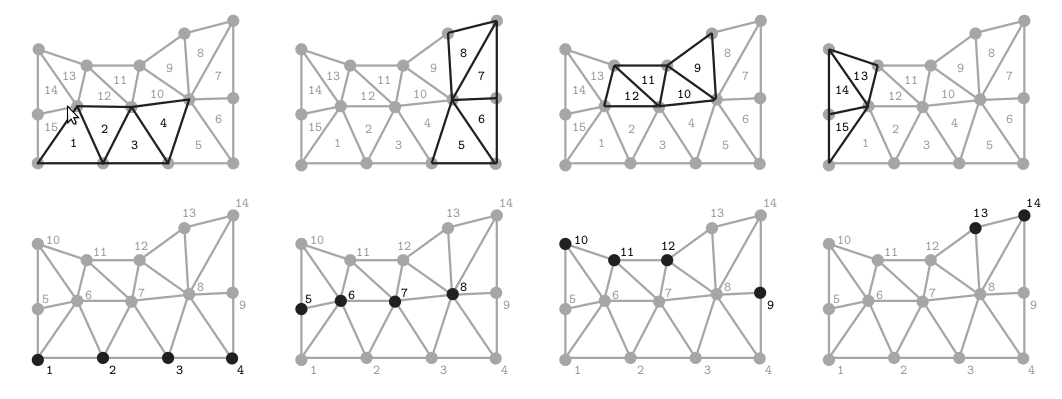
\includegraphics[scale=0.5]{./issue1.png}
\caption{Division of elements and nodes \cite{pccm}}
\begin{picture}(400,0)
\put(40,180){$P0$}
\put(140,180){$P1$}
\put(240,180){$P2$}
\put(340,180){$P3$}
\end{picture}
\end{figure}

In the second approach (Fig. 16, 18), the mesh data is preprocessed. This is done to generate the separate mesh data for each processor so that it has all the elements and node information available. In this case, the serial code needs the least modification. The processors need to communicate the data for the nodes which are common the multiple processors in solver part only. The rest of the parts from serial code can be directly used as they are. This approach is useful because once we have distributed mesh, the same mesh can be reused again and again for parameter studies. It involves one time overhead of generating distributed mesh data. However, this preprocessing takes time for high resolution meshes to be distributed on less number of processors. 

\begin{figure}[!htb]
\centering
\minipage{0.25\textwidth}
\centering
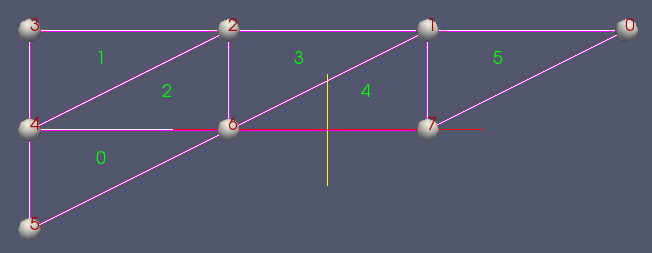
\includegraphics[scale=0.15]{./p0.png}

\textbf{P0}
\endminipage\hfill
\centering
\minipage{0.25\textwidth}
\centering
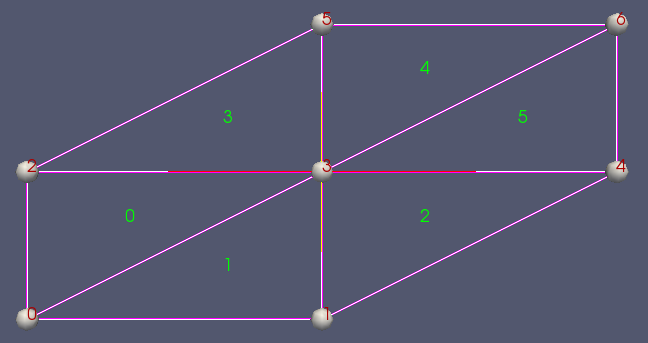
\includegraphics[scale=0.115]{./p1.png}

\textbf{P1}
\endminipage\hfill
\centering
\minipage{0.25\textwidth}
\centering
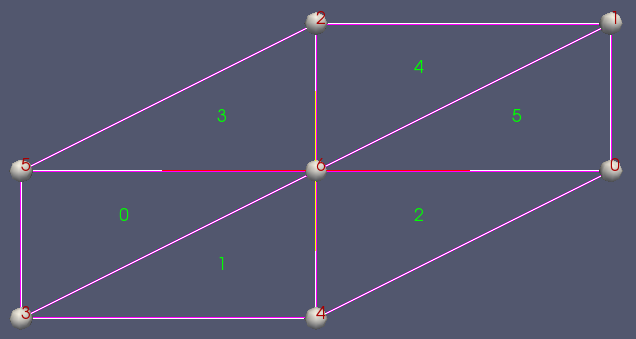
\includegraphics[scale=0.115]{./p2.png}

\textbf{P2}
\endminipage\hfill
\centering
\minipage{0.25\textwidth}
\centering
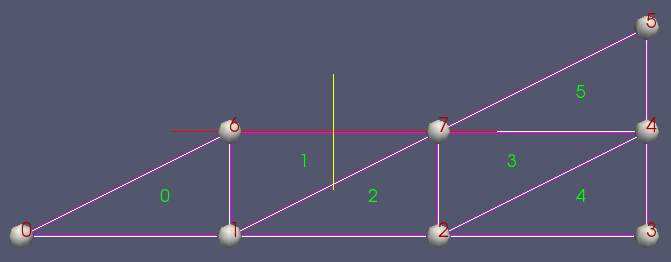
\includegraphics[scale=0.15]{./p3.png}

\textbf{P3}
\endminipage\hfill

\centering 
\caption{Decomposition into separate chunks}
\end{figure}

We have followed second approach in our code because once we have a distributed mesh from a preprocessor, the communication overhead is reduced significantly. We can reuse the distributed mesh for further study of the problem using different boundary conditions. We expect good scalability with this approach.

\section{Mesh Partitioning}
Before the mesh can be used efficiently in parallel, another important process has to be performed over it i.e. Mesh partitioning (Fig. 19, 20). Mesh partitioning is a process of dividing the generated mesh into subdomains. These subdomains can be mapped onto a processor of a parallel machine. The primary goal of mesh partitioning is to minimize communication while maintaining load balance. The communication is associated with the nodes that lie on the boundaries between subdomains and are shared by more than one processor. Processors sharing a node must communicate. Communication time depends on both the message sizes, which increase with the number of shared nodes, and the number of messages, which increases with the number of adjacent subdomains. The load can be predicted to be proportional to the number of nodes on that processor. Prediction becomes more difficult when nonlinearities are present. In these cases, the work per node is solution-dependent. 

The partitioners are based on following algorithms:
 Greedy, Kernighan-Lin, Recursive Coordinate Bisection, Recursive Spectral Bisection, Recursive Inertia Partition, Recursive Graph Bisection, algorithm of Miller, Teng, Thurston, and Vavasis, and Simulated Annealingthe. Miller, Teng, Thurston, and Vavasis algorithm uses geometric information to construct a separator, i.e. a set of nodes whose removal separates the mesh into two pieces of roughly equal size. Each of these pieces is then recursively partitioned until the desired number of subdomains is reached. The Miller algorithm, in practice, rapidly produces high quality partitions. 
 
\begin{figure}[!htb]
\centering
\minipage{0.5\textwidth}
\centering
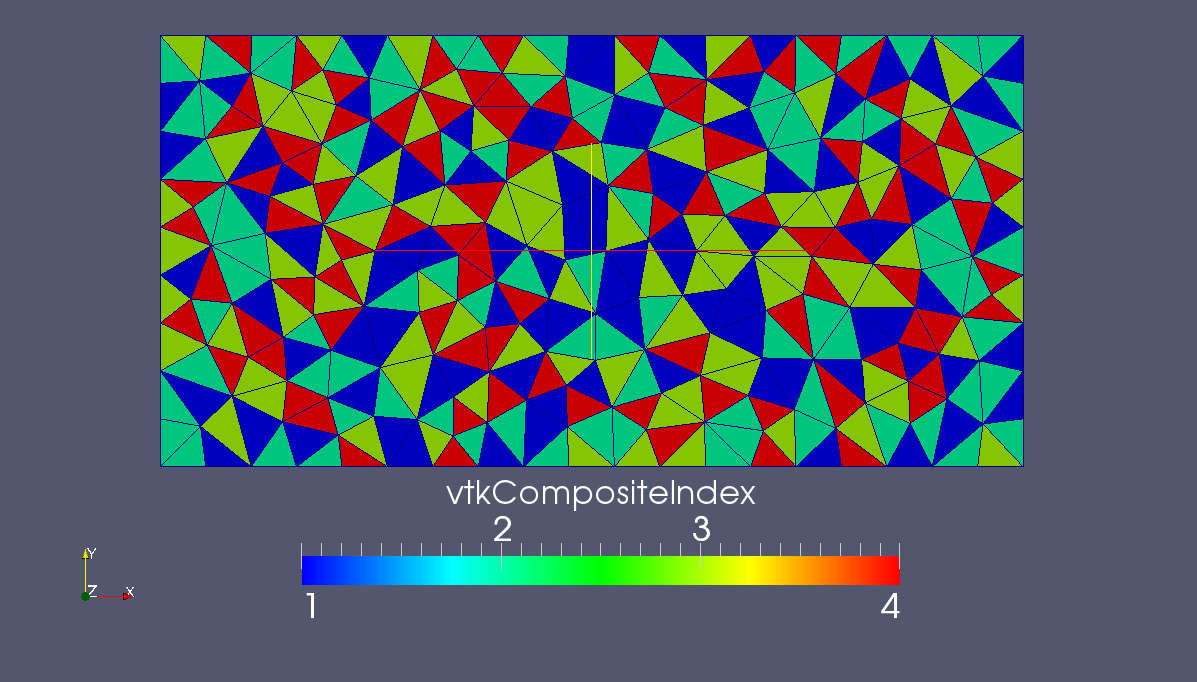
\includegraphics[scale=0.2]{./beforePartition.png}
\caption{Before Mesh partitioning}
\endminipage\hfill
\centering
\minipage{0.5\textwidth}
\centering
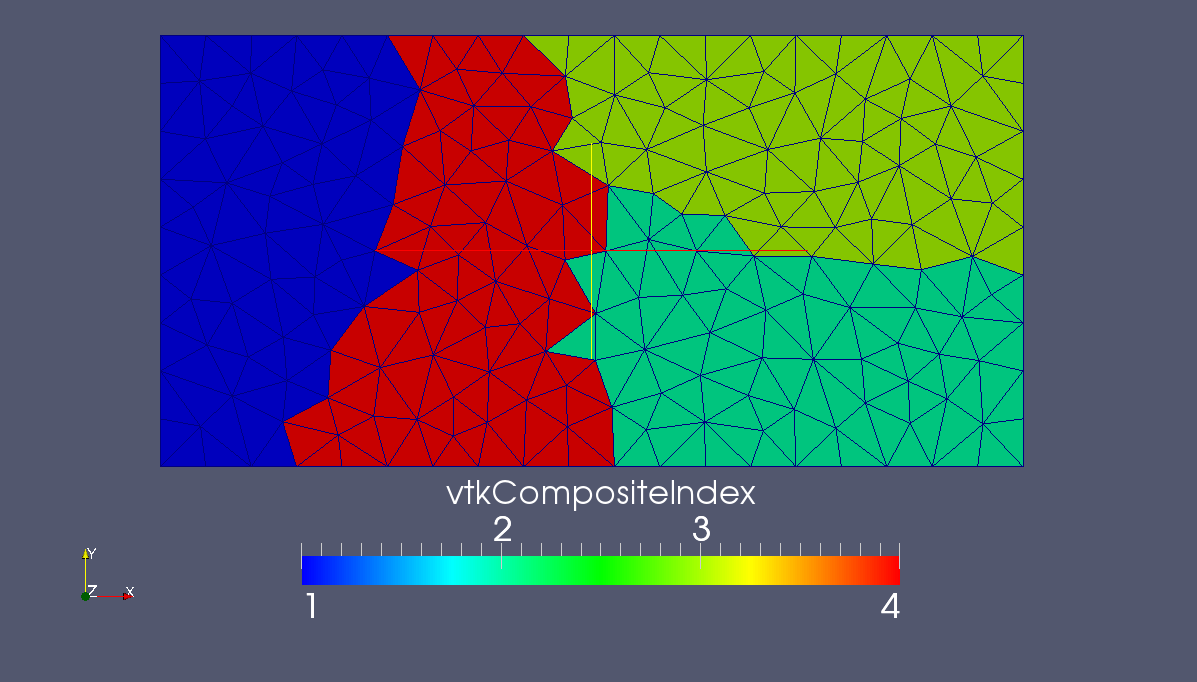
\includegraphics[scale=.2]{./afterPartition.png}
\caption{After Mesh partitioning}
\endminipage\hfill

\end{figure}
 
A typical graph partitioning algorithm finds a decomposition of the graph(non-weighted) with preferably the same number of nodes within each partition and with a minimal number of edges between the partitions. 

There are many public mesh partitioning tools. Some of which are listed below:
\begin{enumerate}
\item METIS
\item TOP/DOMDEC
\item HARP
\item CHACO
\item JOSTLE
\item SCOTCH
\end{enumerate}

In this project, a partition utility is used to partition the usual mien FEM connectivity into a set of contiguous subdomains using the Metis graph partitioning library available on cluster. This generates a mprm file which is used in subsequent preprocessing of mesh.

\section{Preprocessor}
The preprocessor takes the raw mxyz, mien, minf, mrng files and decomposes them according to the partitioning defined in mprm file into number of processors specified in "settings.in". This is a serial program. 
It generates an additional file "procb" which contains the information of nodes shared among the processors. This file contains following information per node: global node number, how many processors it is shared with, array of the processor ranks it is shared with. If the node is not shared with any other processor, the array has default value of -1.
Sample procb file for $proc\_0$ is shown below:

\begin{center}

\begin{tabular}{cccccc}

0 & 0 & -1 & -1 & -1 & -1 \\ 

1 & 0 & -1 & -1 & -1 & -1 \\ 

2 & 0 & -1 & -1 & -1 & -1 \\ 

3 & 1 & 1 & -1 & -1 & -1 \\ 

13 & 1 & 1 & -1 & -1 & -1 \\ 

14 & 1 & 1 & -1 & -1 & -1 \\ 
 
15 & 2 & 1 & 2 & -1 & -1 \\ 
 
16 & 2 & 1 & 2 & -1 & -1 \\ 
\end{tabular} 

 \text{Contents of a sample procb file}
\end{center}

% Define the styles for each block
\tikzstyle{startstop} = [rectangle, rounded corners, minimum width=3cm, minimum height=1cm,text centered, draw=black, fill=red!30]
\tikzstyle{io} = [trapezium, trapezium left angle=70, trapezium right angle=110, minimum width=3cm, minimum height=1cm, text centered, draw=black, fill=blue!30]
\tikzstyle{process} = [rectangle, minimum width=3cm, minimum height=1cm, text centered, draw=black, fill=orange!30]
\tikzstyle{decision} = [diamond, minimum width=3cm, minimum height=1cm, text centered, draw=black, fill=green!30]
\tikzstyle{arrow} = [thick,->,>=stealth]
\begin{figure}
\begin{center}
\begin{tikzpicture}[node distance=2cm]

% Nodes
\node (start) [startstop] {Start};

\node (in1) [io, below of=start, minimum width=2cm, minimum height=1cm, text centered, text width=6cm, draw=black, yshift=-0.5cm] {Read: Mesh files: mxyz, mien, minf, mrng, mprm, Input file: settings.in (no. of procs)};

\node (pro1) [process, below of=in1, yshift=-0.5cm] {Define Mesh Structures per processor};

\node (pro2) [process, below of=pro1, minimum width=5cm, minimum height=1cm, text centered, text width=5cm, draw=black] {Distribute the elements and nodes per processor based on partitioning};

\node (pro2z) [process, below of=pro2, minimum width=6cm, minimum height=1cm, text centered, text width=6cm, draw=black] {Generate mxyz,mien,minf,mrng and procb files per processor};

\node (stop) [startstop, below of=pro2z] {Stop};

% Arrows
\draw [arrow] (start) -- (in1);
\draw [arrow] (in1) -- (pro1);
\draw [arrow] (pro1) -- (pro2);
\draw [arrow] (pro2) -- (pro2z);
\draw [arrow] (pro2z) -- (stop);

\end{tikzpicture}\\
\end{center}
\caption{Preprocessor Flow Chart}
\end{figure}

\section{Overall Flow of program}
Overall program flow is shown in Figure 22. Each processors runs through the steps shown in the flowchart. This generates VTK data per time step for each processor separately.

%<TikZ code>
\begin{figure}

\begin{center}
\begin{tikzpicture}[node distance=2cm]

% Nodes
\node (start) [startstop] {Start};

\node (in1) [io, below of=start, minimum width=2cm, minimum height=1cm, text centered, text width=6cm, draw=black, yshift=-0.5cm] {Input: Preprocessed Mesh files, Initial and Boundary conditions, Diffusion Coefficient, Source term, No. of iterations, Time step, Data Writing Frequency};

\node (pro1) [process, below of=in1, yshift=-0.5cm] {Define Mesh Structures};
\node (pro2) [process, below of=pro1, minimum width=5cm, minimum height=1cm, text centered, text width=5cm, draw=black] {Calculate Metrics: Jacobian, Element level Matrices};

\node (pro2z) [process, below of=pro2, minimum width=4cm, minimum height=1cm, text centered, text width=3cm, draw=black] {Apply Boundary Conditions};
%\node (dec1) [decision, below of=pro1, yshift=-0.5cm] {Decision 1};

\node (pro2a) [process, below of=pro2z,  minimum width=3cm, minimum height=1cm, text centered, text width=5cm, draw=black] {Solver: Assembly of M and RHS};

\node (pro2aa) [process, below of=pro2a,  minimum width=3cm, minimum height=1cm, text centered, text width=5cm, draw=black] {Solver: MPI Communication of M and RHS for shared nodes among the processors};

\node (pro2ab) [process, below of=pro2aa,  minimum width=3cm, minimum height=1cm, text centered, text width=5cm, draw=black] {Solver: Solve for Temperature [M]\{T\} = \{RHS\}};

\node (pro2b) [io, below of=pro2ab, minimum width=3cm, minimum height=1cm, text centered, text width=2cm, draw=black] {Write VTK Data};

\node (pro2c) [process, right of=pro2b, xshift=2cm] {time+=dt};
\node (dec1) [decision, below of=pro2b, yshift=-0.5cm] {iter<NIter};
%\node (out1) [io, below of=dec1, yshift=-0.5cm, minimum width=3cm, minimum height=1cm, text centered, text width=3cm, draw=black] {Output in Paraview};

\node (stop) [startstop, below of=dec1, yshift=-0.5cm] {Stop};

% Arrows
\draw [arrow] (start) -- (in1);
\draw [arrow] (in1) -- (pro1);
\draw [arrow] (pro1) -- (pro2);
\draw [arrow] (pro2) -- (pro2z);
\draw [arrow] (pro2z) -- (pro2a);
\draw [arrow] (pro2a) -- (pro2aa);
\draw [arrow] (pro2aa) -- (pro2ab);
\draw [arrow] (pro2ab) -- (pro2b);
\draw [arrow] (pro2b) -- (dec1);
\draw [arrow] (dec1) -- node[anchor=east] {no} (stop);
\draw [arrow] (dec1) -| node[anchor=south] {yes} (pro2c);
\draw [arrow] (pro2c) |- (pro2a);
%\draw [arrow] (out1) -- (stop);

\end{tikzpicture}\\
\end{center}
\caption{Overall Program Flow Chart}
\end{figure}


\section{MPI Communication}
Each of the processor reads its portion of mesh, calculates jacobian for each element, assembles element level matrices and finally in solver part assembles the lumped mass matrix (M) and right hand side vector (RHS) of the equation to be solved. However, for the nodes which are shared between different processors, these assembled entities still need the contribution from elements on the other processors. This information needs to be communicated between the concerned processors before the equation can be solved. The procb file which is generated by preprocessor comes into play here. 

Two side communication has been used. The communication is initiated by each of the processors based on the procb file. For the node which is shared between the two processors, the data i.e. M and RHS for the corresponding node is exchanged. On the receiving processor, the addition of received M and RHS to the correct location of existing M and RHS is achieved by matching the global node number.

\section{Parallel Results}
\subsection{Verification}
Verification of parallel code is necessary to check if the code is really doing what the physics of the problem states rather than just solving the problem faster. We validate the parallel code versus the results from serial code as the later has been already validated. A rectangular domain is considered for heat diffusion problem. Left and bottom walls are kept at 1000 K while top and right walls are maintained at 300 K and the temperature profile is allowed to develop over time. The temperature values along the diagonal line shown in Fig. 22 are compared for serial and parallel code The snapshots are taken at t = 0.001 s, t = 0.01 s, t = 0.1 s. From Figure 23, it can be seen that they match one to one for all times. This concludes the verification of parallel code.

\begin{figure}[!htb]
\centering
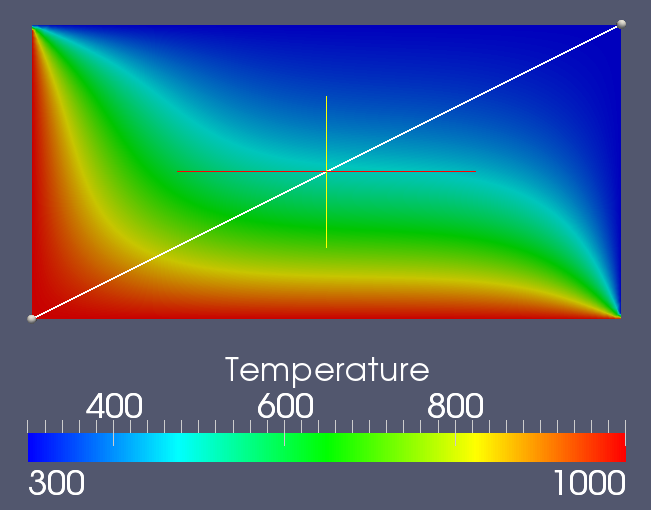
\includegraphics[scale=0.6]{./verification_paraview.png}
\caption{Temperature distribution at t = 0.1 s for np = 4}
\end{figure}
\begin{figure}[!htb]
\centering
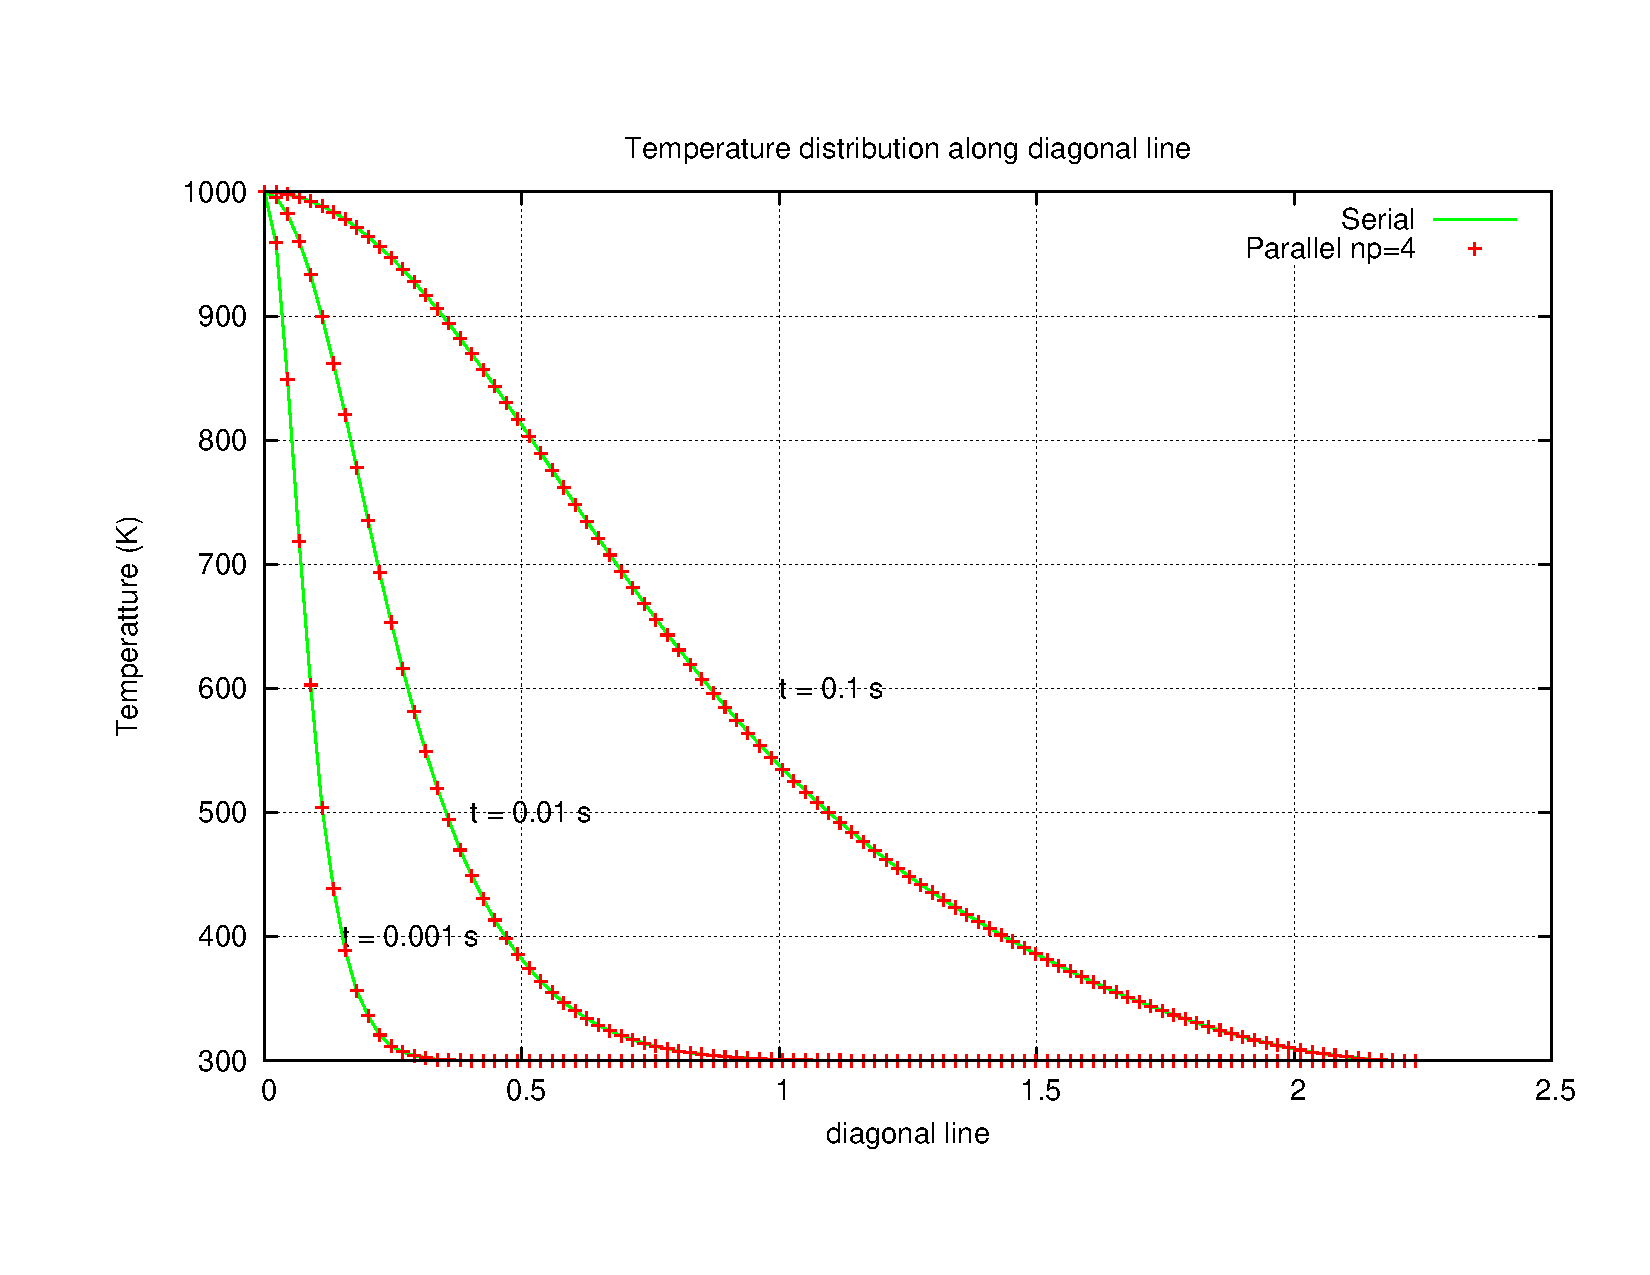
\includegraphics[scale=0.6]{./verification_par.pdf}
\caption{Comparison of Serial and Parallel results}
\end{figure}

\subsection{Scalability}
Scalability studies are performed to see if it is beneficial at all to use the parallel code compared to serial code. The parallel code should run faster for the same problem size with increasing number of processors. This is called strong scaling. Figure 25 shows the speedup obtained for finest mesh from Rectangular domain while Figure 26 shows the speedup obtained for superfine mesh. The parallelized code shows some scalability though it is not very close to ideal linear one. The divergence from the linear graph is due to the increasing communication overhead. The performance begins to drop after 256 cores. As the given domain is divided into more and more smaller parts, there are more number of nodes which are on the boundaries between the processors which increases the send/recv messages. Ideally, the code should give better results if the percentage of boundary nodes is well below the percentage of inner nodes. 

\begin{figure}[!htb]
\centering
\minipage{0.5\textwidth}
\centering
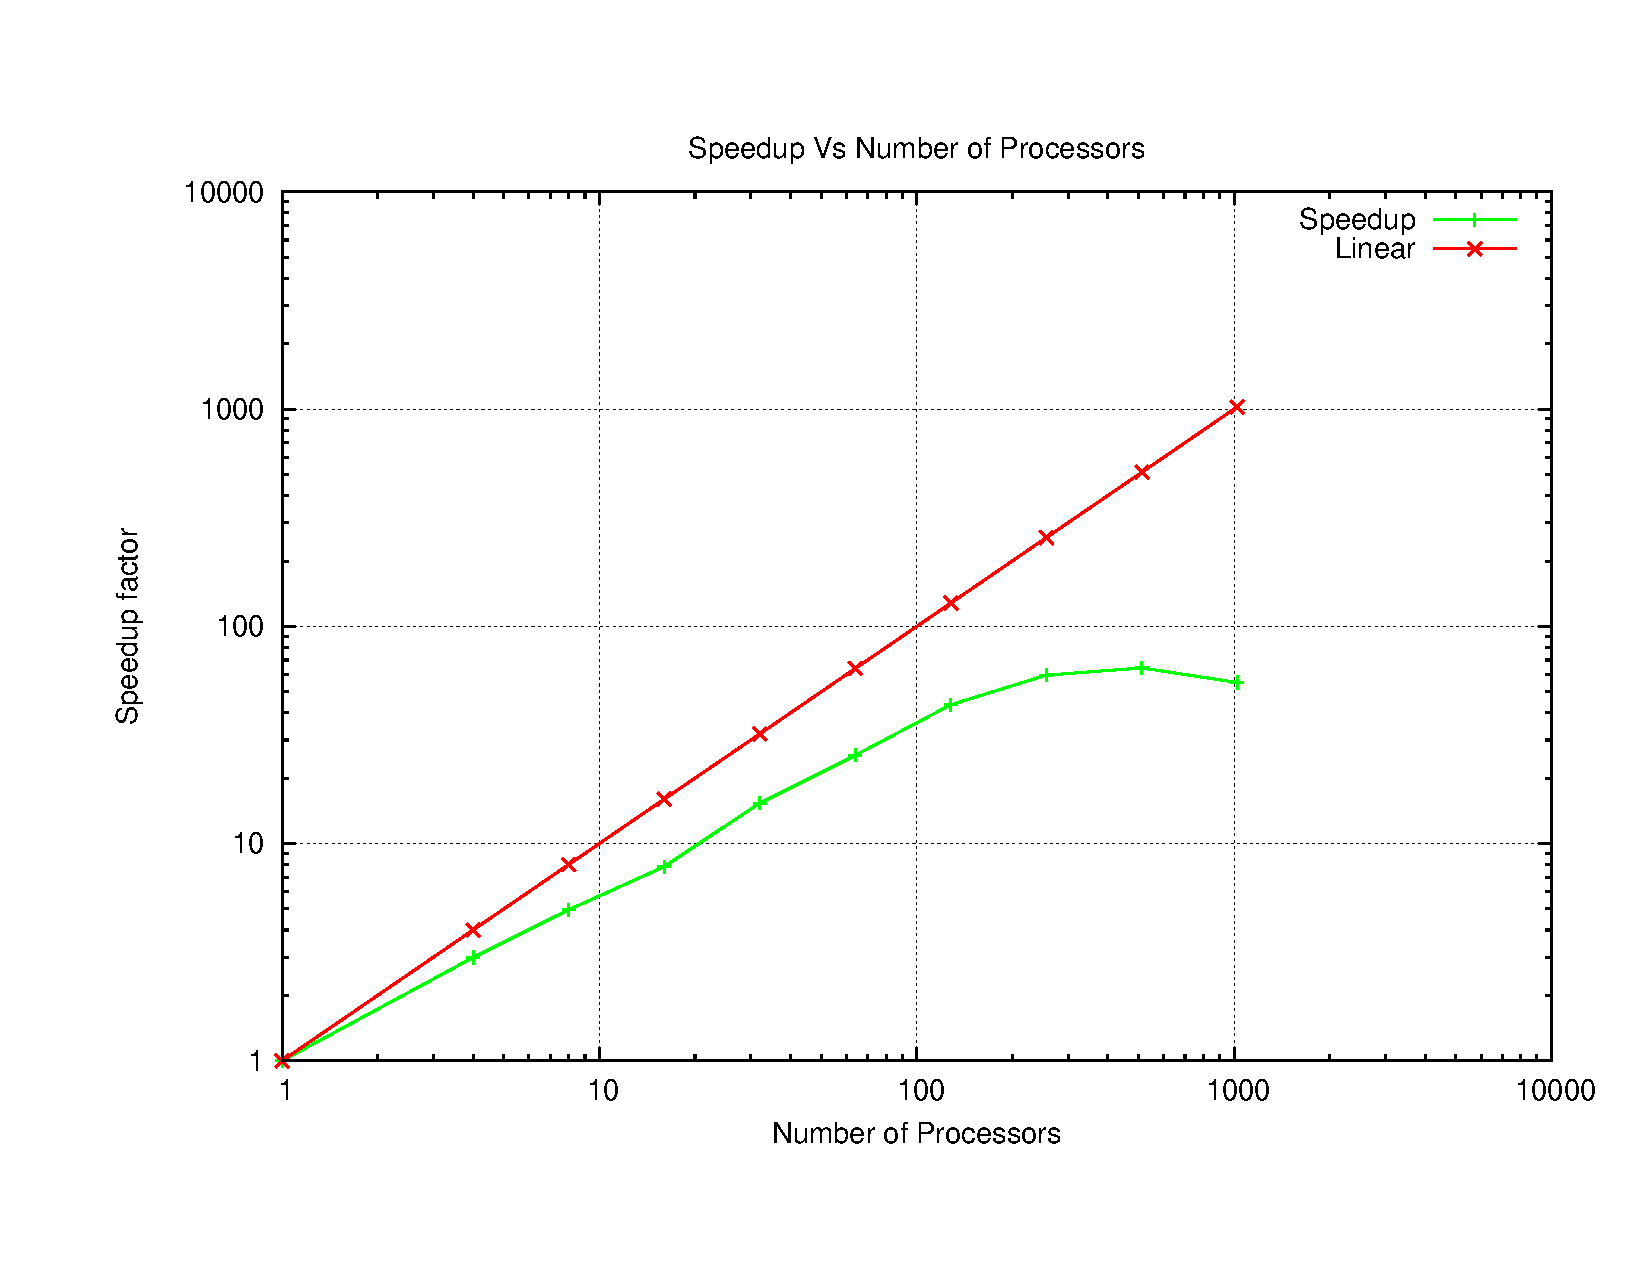
\includegraphics[scale=0.33]{./Timings_1.pdf}
\centering
\caption{Finestmesh: ne = 516160, nn = 259082}
\endminipage\hfill
\centering
\minipage{0.5\textwidth}
\centering
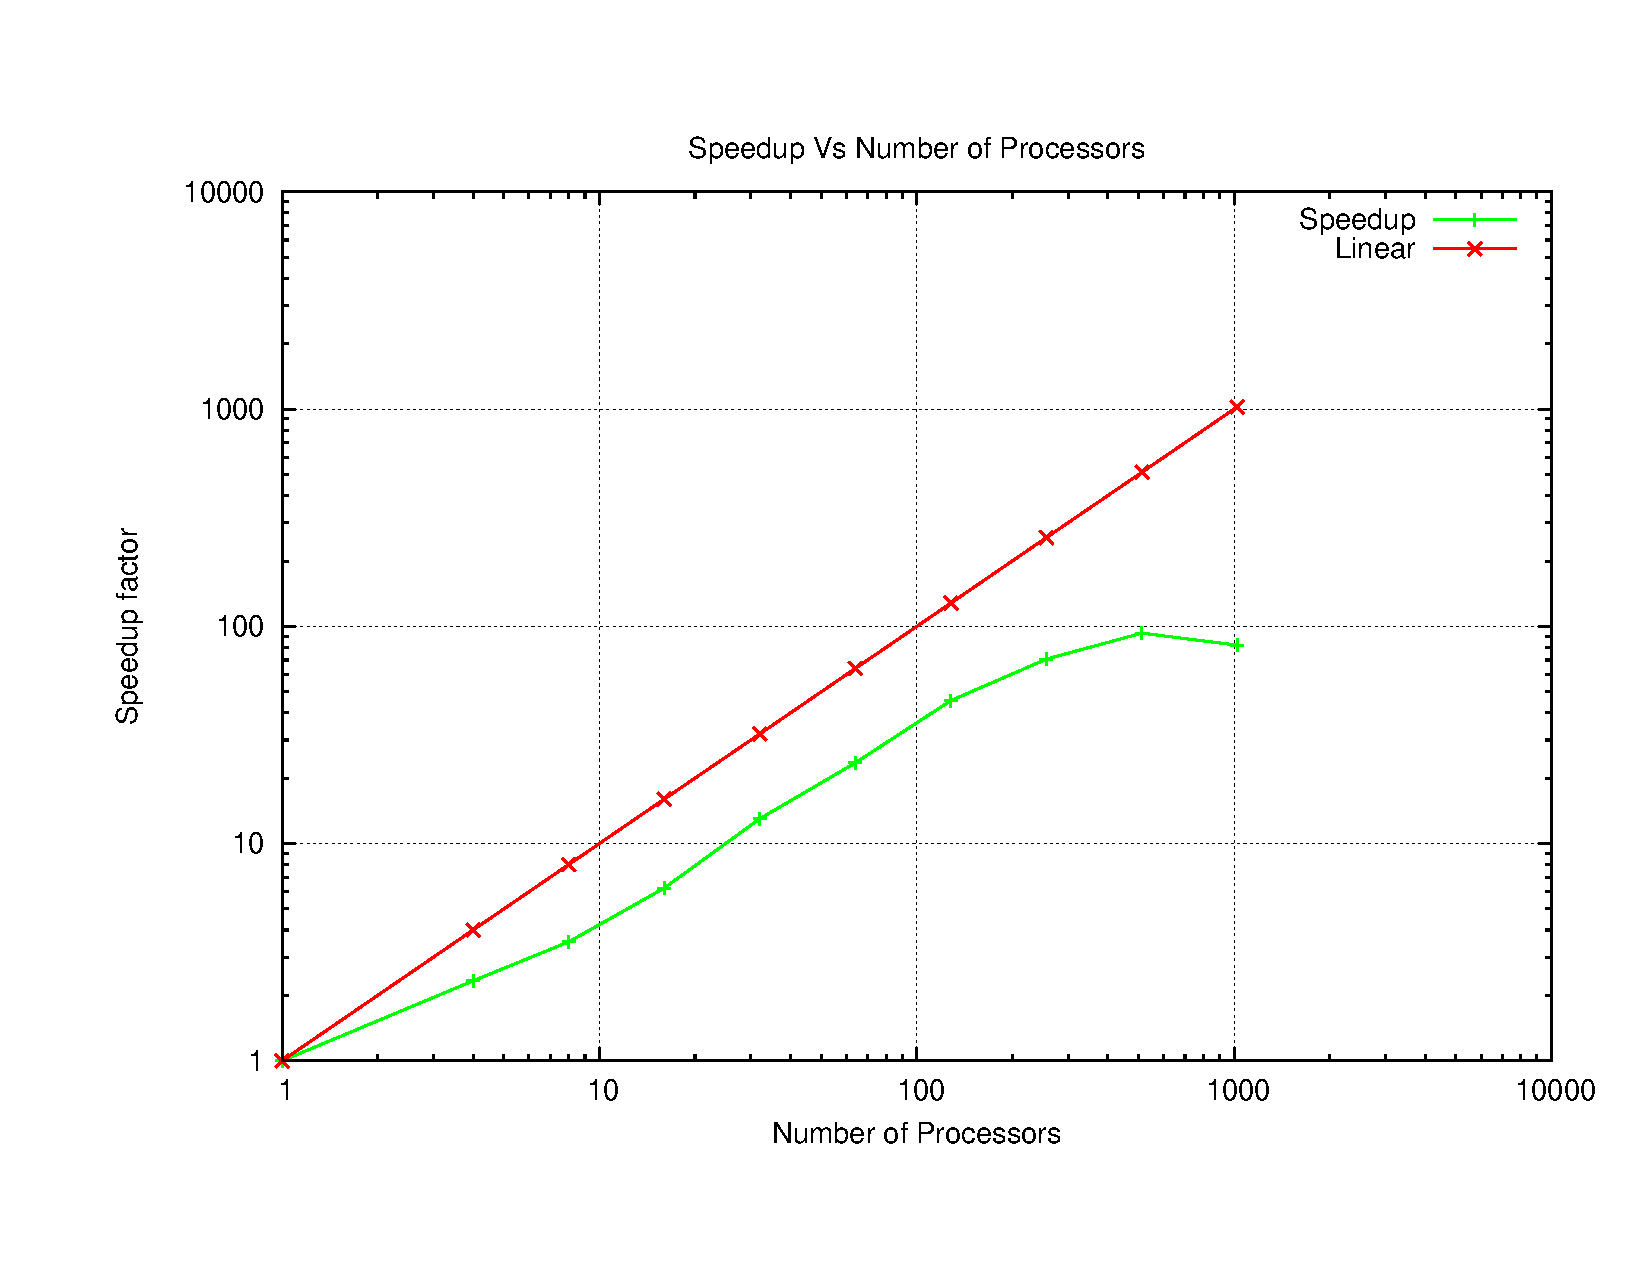
\includegraphics[scale=0.33]{./Timings_2.pdf}
\centering
\caption{Superfine: ne = 945746, nn = 474074}
\endminipage\hfill
\end{figure}

\subsection{Scalasca}
SCALASCA is an open-source toolset for scalable performance analysis of large-scale parallel applications. We tried to analyse our parallel code using scalasca. We can see the screenshot in Figure 27. It shows the how the communication time is distributed among the processors. One processor takes more time for the communication. This might happen if the processor has more number of boundary nodes than other processors. 
\begin{figure}[!htb]
\centering
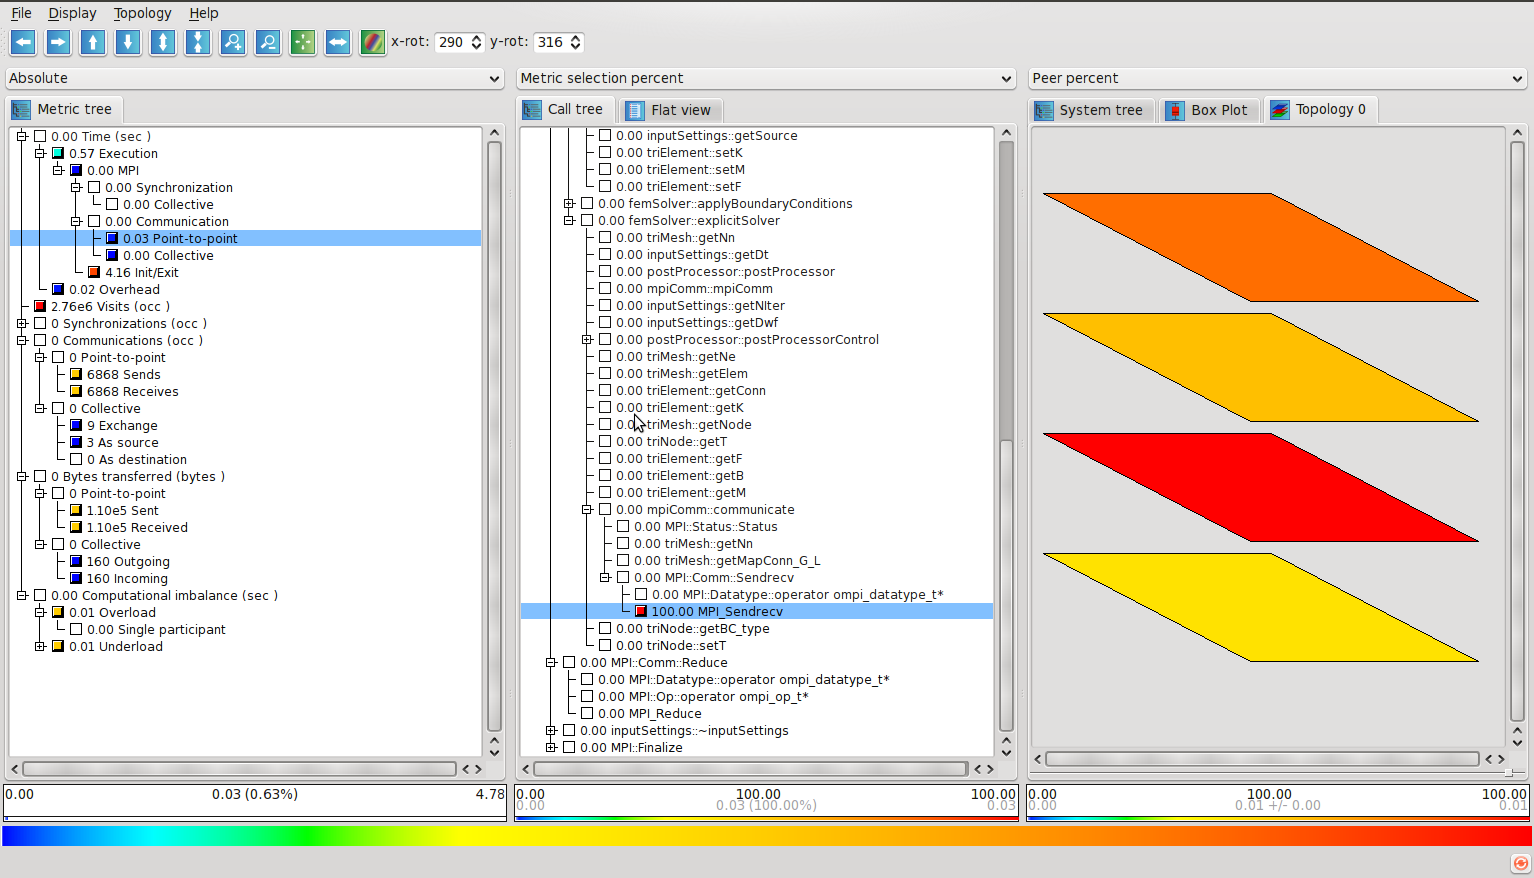
\includegraphics[scale=0.4]{./scalasca.png}
\caption{Screenshot of Scalasca np = 4}
\end{figure}

\section{Application}
The working parallel code is directly applied to a realistic problem. The problem is defined as follows:
Performance of the microprocessors improved significantly over last two decades in agreement with the Moore's Law. In order to achieve this improvement, more and more transistors are packed  into the same area of the chip increasing the performance as well as the heat sinks fail to satisfy this increasing cooling demand. One of the remedies to manage microprocessor power dissipation is the use of microchannels, which offers very high heat transfer rates in a very small area.

A heat sink for cooling computer chip, which is fabricated from copper with machined microchannels, is shown in Figure 28. Within these microchannels, water flows and carries away the heat dissipated by the chips. The lower side of the sink is insulated while the upper side is exposed to ambient air. When we consider the symmetric unit on the right side of the Figure 28, it is possible to treat the right and left surfaces as insulated boundaries.
\begin{figure}[!htb]
\centering
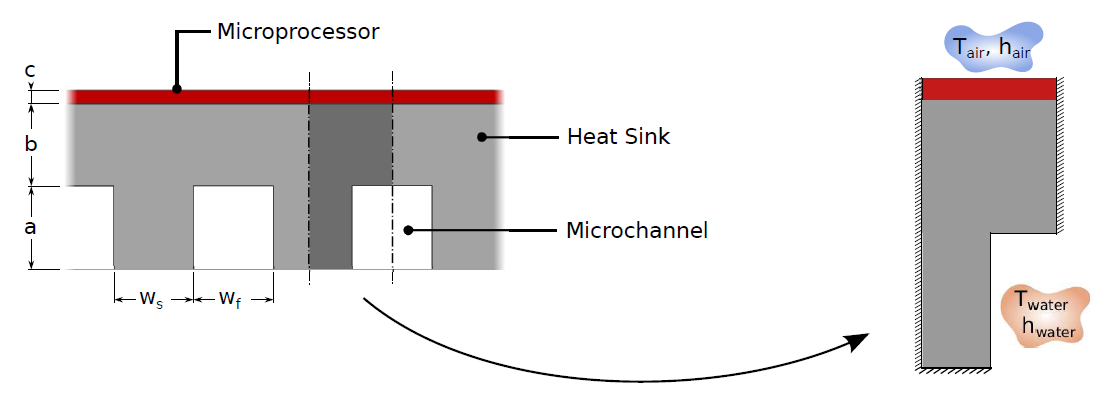
\includegraphics[scale=0.5]{./application.png}
\caption{Illustration of the heat sink and the symmetric region}
\end{figure}

Physical properties and dimensions:

\begin{itemize}
\item Dimensions of the heat sink: a = b = $w_s$ = $w_f$ = 0.2 mm, c = 0.02 mm
\item Thermal diffusivity of copper: $\alpha_{copper}$ = 1.11 $\times$ $10^{-4}$ $m^2/s$
\item Density of copper: $\rho$ = 8940 $kg/m^3$
\item Specific heat capacity: $C_p$ = 385 J/kg/K
\item Properties of cooling fluid: $T_{water}$ = $25^o$ C, $h_{water}$ = 30000 $W/m^2/K$
\item Properties of ambient air: $T_{air}$ = $25^o$ C, $h_{air}$ = 2 $W/m^2/K$
\end{itemize}
Using the given mesh file, physical properties and dimensions, solve for the following cases:

\subsection*{Case 1}

To understand the physics of the problem, we can start with a simplified approach. Suppose that there is no heat generation in the microprocessor and assume that the top surface is kept at constant temperature of T = $75^o$C instead of being exposed to the ambient air. Determine the steady state temperature distribution in the heat sink and the time required to reach steady state conditions.

The steady state criteria is defined as the maximum rate of change of temperature in the domain $$\left(\frac{dT}{dt}\right)_{max} \leq 0.001$$

The temperature distribution reaches steady state in \textbf{8.4237117 ms}. The distribution can be seen in Figure 29. The dynamics of the system are very fast as the copper is good conductor of heat. The gradient inside the heat sink is more or less $3^o C$.
\begin{figure}[!htb]
\centering
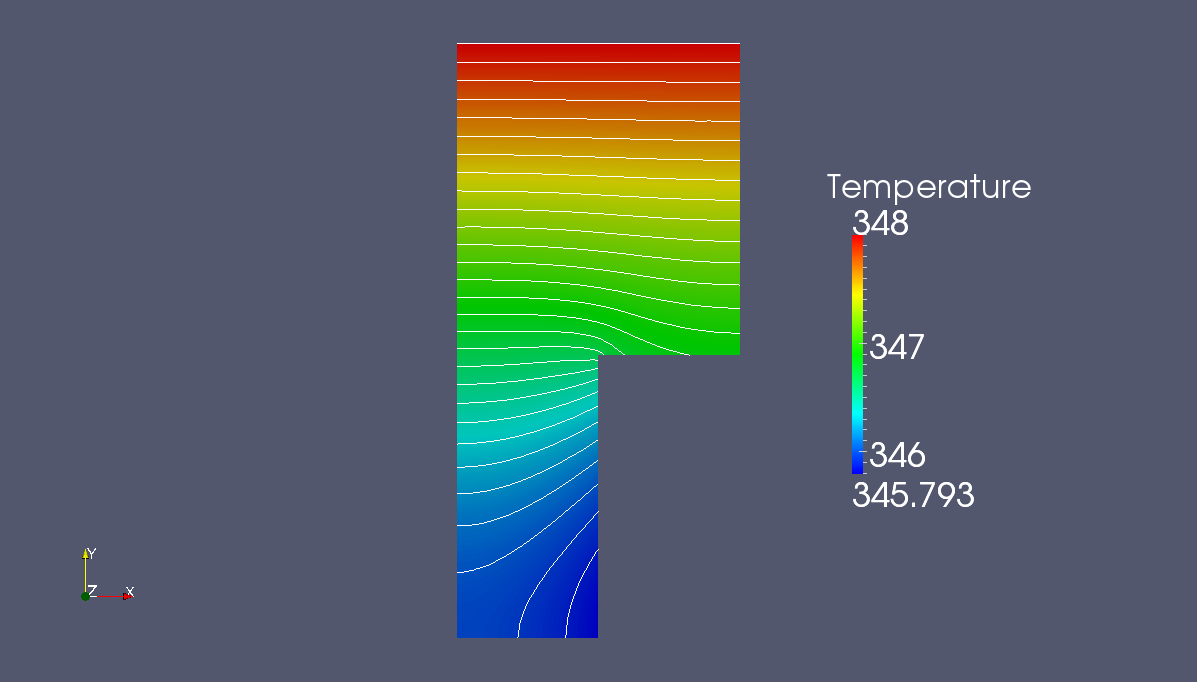
\includegraphics[scale=0.3]{./case1_c.png}
\caption{Steady state temperature distribution in Case 1}
\end{figure}

\subsection*{Case 2}

Having obtained an idea about the physics of th e problem, we can concentrate on the real problem.

(a) Now suppose that the microprocessor is generating heat and the top surface is exposed to ambient air. Given the maximum allowable temperature in the microprocessor is T = $75^o$ C, determine how much the maximum possible heat generation rate in the chips can be. 

We can use the result of case 1 as the initial condition. 

The maximum heat generation rate in the chip obtained by solving the problem is approximately \textbf{9.6 $\times$ $10^{10}$ $W/m^3$}. If we consider a chip of dimensions $10$ mm$\times10$ mm, it is allowed to generate maximum \textbf{192 W} of heat so that the temperature in the chip doesn't exceed $75^o$ C. This is a reasonable amount of heat dissipation given that the chip is water cooled. 

(b) Using maximum heat generation rate found in part (a), determine the steady state temperature distribution in the heat sink and time required to reach the steady state.

Figure 30 shows the steady state temperature distribution in the heat sink when there is heat generation. If we compare the distribution in case 2 with case 1, there is not so much difference except that the isolines in the heat generation region are curved depending on the nature of diffusion. The lowest temperature values differ slightly. The time required to reach the steady state is more than 10 ms. 

 
\begin{figure}[!htb]
\centering
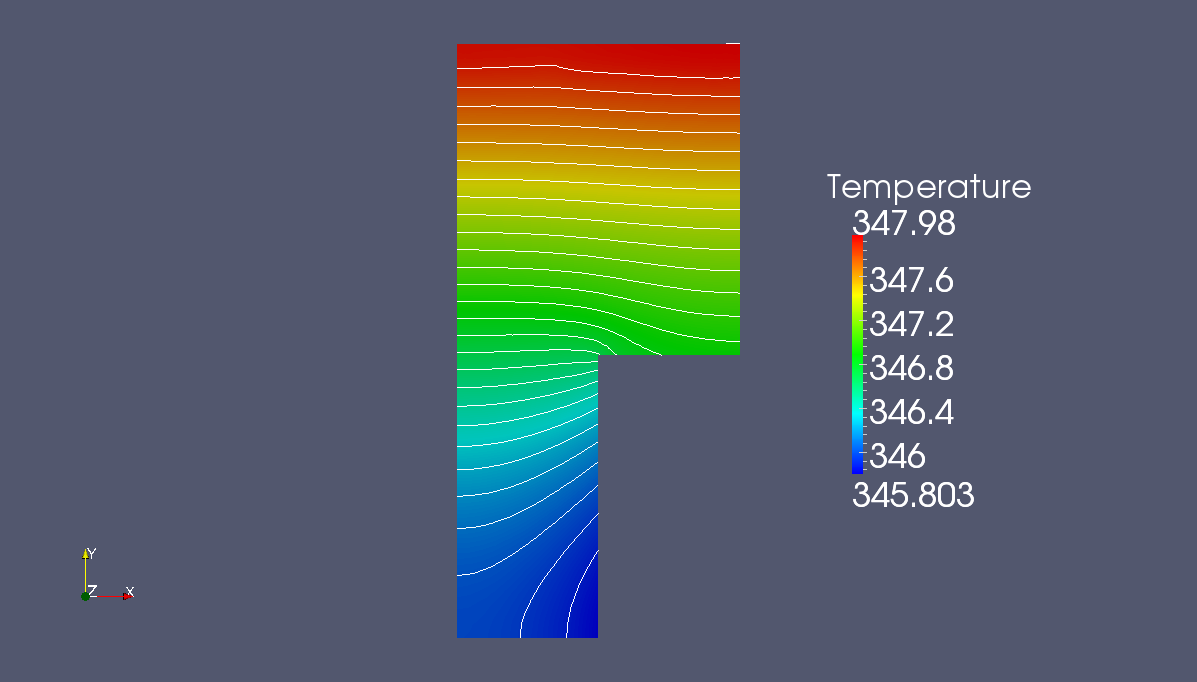
\includegraphics[scale=0.3]{./case2_c.png}
\caption{Steady state temperature distribution in Case 2}
\end{figure}


\section{Summary}
A two dimensional transient heat diffusion equation is solved numerically using finite element method on unstructured mesh. The FEM uses triangular linear elements. A serial object oriented C++ code is developed based on the FE formulation described in earlier sections. The code is verified against analytical solutions found in \cite{jw}. A parallel code is also developed to be able to solve larger problems faster. The parallel code shows sufficient amount of scalability. Finally, the capability of the software to be applied to a realistic problem has been demonstrated.

\bibliographystyle{unsrt}
\bibliography{literature}

\end{document}
